\documentclass[11pt]{report}

\usepackage{times}
\usepackage{latexsym}
\usepackage{booktabs}
\usepackage{amsmath}
\usepackage{multirow}
\usepackage{enumitem}
\usepackage{amsfonts}
\DeclareMathOperator*{\argmax}{arg\,max}

\newcommand{\Correct}{\checktikz[draw=black]}
\newcommand{\ValidMiss}{\checktikz[draw=gray,fill=white]}
\newcommand{\Valid}{\checktikz[draw=gray,fill=white]}
\newcommand{\Missed}{\checktikz[draw=black]} %\textsf{X}~}
\newcommand{\Wrong}{} %\textsf{X}~}

\usepackage[utf8]{inputenc}
\usepackage[letterpaper,bindingoffset=0.2in,%
            left=1in,right=1in,top=1in,bottom=1in,%
            footskip=.25in]{geometry}
\usepackage{microtype}
\usepackage{mathtools}
\usepackage{latexsym, mathrsfs}
\usepackage{graphicx}
\usepackage{subcaption}
\usepackage[usenames,dvipsnames,svgnames,table]{xcolor}
\usepackage[framemethod=TikZ]{mdframed}
\usepackage[linesnumbered,ruled,procnumbered]{algorithm2e}
\usepackage{enumitem}
\usepackage{multirow}
\usepackage{xspace}
\usepackage{textcomp}
\usepackage{setspace}
\usepackage{tikz}
\usepackage{hhline}
\usepackage[numbers,sort]{natbib}
\usepackage[nottoc]{tocbibind}
\usepackage[normalem]{ulem}
\usepackage[titletoc]{appendix}

\usepackage{titlesec}
\titleformat{\chapter}
  {\normalfont\LARGE\bfseries}{\thechapter}{1em}{}
\titlespacing*{\chapter}{0pt}{3.5ex plus 1ex minus .2ex}{2.3ex plus .2ex}

% VQuel listing
\newcommand{\mysinglespacing}{%
  \setstretch{1}% no correction afterwards
}


\usepackage[pdfpagelabels=false]{hyperref}
\hypersetup{
   colorlinks,
   linkcolor={red!50!black},
   citecolor={blue!50!black},
   urlcolor={blue!80!black}
}

\SetAlFnt{\small}

\mdfdefinestyle{MyFrame}{%
    linecolor=black,
    outerlinewidth=1pt,
    roundcorner=10pt,
    innertopmargin=\baselineskip,
    innerbottommargin=\baselineskip,
    innerrightmargin=20pt,
    innerleftmargin=20pt,
    backgroundcolor=gray!50!white}
    
\newenvironment{denselist}{
    \begin{list}{\small{$\bullet$}}%
    {\setlength{\itemsep}{0ex} \setlength{\topsep}{0ex}
    \setlength{\parsep}{0pt} \setlength{\itemindent}{0pt}
    \setlength{\leftmargin}{1.5em}
    \setlength{\partopsep}{0pt}}}%
    {\end{list}}

\usepackage{cleveref}
\crefname{section}{\S\!\!\!\;}{\S\S}
\Crefname{section}{\S}{\S\S}

\RequirePackage{natbib}
% for citation commands in the .tex, authors can use:
% \citep, \citet, and \citeyearpar for compatibility with natbib, or
% \cite, \newcite, and \shortcite for compatibility with older ACL .sty files
\renewcommand\cite{\citep}	% to get "(Author Year)" with natbib    
\newcommand\shortcite{\citeyearpar}% to get "(Year)" with natbib    
\newcommand\newcite{\citet}	% to get "Author (Year)" with natbib   

\newcommand{\topic}[1]{\vspace{-3.5pt}\smallskip \smallskip \noindent{\bf #1:}}
\newcommand{\stitle}[1]{\vspace{0.5em}\noindent\textbf{#1}}
\renewcommand{\stitle}[1]{\vspace{1em}\noindent\textbf{#1}}

\newcommand{\speaker}[1]{{\bf\footnotesize\textsf{#1}}}
\renewcommand{\vec}[1]{\boldsymbol{#1}}

%COMPRESS
\newcommand{\squeezeup}{\vspace{-2.5mm}}

\newcommand{\U}{\mathbb{U}}

\title{
{\bf Teaching Machines to Ask Clarification Questions}\\
\vspace{18pt}
\it Preliminary Oral Exam (Thesis Proposal)}

\author{
{\bf Sudha Rao}  \\
Department of Computer Science \\
University of Maryland, College Park\\
{\texttt{raosudha@cs.umd.edu}}
}


\date{
\vspace{42pt}
Dissertation Proposal submitted to: \\
Department of Computer Science \\
University of Maryland, College Park, MD 20742 \\
\bigskip
\bigskip
\today
\bigskip
\bigskip
\begin{table}[htp]
\begin{center}
\begin{tabular}{lll}
&\multicolumn{2}{l}{Advisory Committee:} \\ \\
Dr. Hal Daum\`{e} III & Chair & U. of Maryland, College Park \\
Dr. David Jacobs & Dept's Rep & U. of Maryland, College Park \\
Dr. Philip Resnik & Member & U. of Maryland, College Park \\
Dr. Lucy Vanderwende & Member & Microsoft Research \\
\end{tabular}
\end{center}
\end{table}%
}


\begin{document}

\pagestyle{plain}
\pagenumbering{roman}

\maketitle
\pagebreak

\begin{abstract}
\normalsize

Inquiry is fundamental to communication, and machines cannot effectively collaborate with humans unless they can ask questions. Asking questions is also a natural way for machines to express uncertainty, a task of increasing importance in an automated society. In the field of natural language processing, despite decades of work on question answering, there is relatively little work in question asking. Moreover, most of the previous work has focused on generating reading comprehension style questions which are answerable from the provided text. The goal of my dissertation work, on the other hand, is to teach machines to ask clarification questions pointing out the missing information in a text. Primarily, I focus on two scenarios where I find such question asking to be useful: (1) clarification questions on posts found in community-driven Q\&A forums like StackExchange (2) clarification questions during goal-oriented dialogue sessions. 

In my first line of research, I study the problem of question generation using data from StackExchange, a plentiful online resource in which people routinely ask clarifying questions to posts so that they can better offer assistance to the original poster. In my preliminary work, I created a novel dataset using StackExchange and addressed the question selection problem, more specifically select the right clarification question from a set of prior questions. I developed a novel neural network model inspired by the notion of expected value of perfect information: a good question is the one whose expected answer is going to be the most useful. In my first proposed work, I plan to use the following two strategies to build more generalizable systems: (a) a template based question generation model and (b) an encoder-decoder based neural generative model.

In my second line of research, I study the problem of question generation using the Ubuntu Dialogue Corpus, a two-way conversational data extracted systematically from chat logs where people discuss issues with their Ubuntu Operating system. In my preliminary work, I addressed the task of predicting the next best response given a context of a conversation. I built a novel neural network model inspired by the best practices in dialogue modeling coupled with our novel vocabulary selection strategies. In my second proposed work, I plan to explore how can I generate a clarification question as the next response, given different levels of context of a conversation. 

In both the research agendas described so far, I took a purely corpus-driven approach to generating clarification questions i.e. learning to ask a question by looking at previously asked questions in a similar context. However, inferring a knowledge gap requires a certain level of domain knowledge that is currently lacking in our proposed models. Therefore, in my third proposed work, I plan to explore how can we use external knowledge sources to understand what is missing in a given context and then ask a clarification question. 

\end{abstract}

\pagebreak

\tableofcontents
\pagebreak

\cleardoublepage
\pagenumbering{arabic}


\chapter{Introduction}

\section{Motivation}

An overarching goal of the natural language processing community is to develop techniques that would enable machines to process naturally occurring text as efficiently as humans do. However, as humans, we do not always understand each other. According to Gricean pragmatics \cite{grice1975logic}, speakers and listeners adhere to a Cooperative Principle where a speaker communicates information that is as informative as required and not more. In case of gaps or mismatches in knowledge, the listener resorts to asking questions. With the advancements of artificial intelligence technologies, we increasingly find ourselves interacting with automated agents (like Apple's Siri, Amazon's Alexa, Google Home, etc) in naturally spoken languages. If we wish to make such human-bot interactions as efficient as human-human interactions are, it is important that we teach machines to ask clarification questions when faced with uncertainty or knowledge gaps.\\

\noindent
In the field of natural language processing, however, despite decades of work on question answering, there has been little work in question asking. Moreover most of the previous work on generating questions has been on generating reading comprehension style questions: given a text, write a question that one might find on a standardized test assessing the knowledge of a student about a particular topic in the text. Comprehension questions, by definition, are answerable from the provided text. Clarification questions are not. The goal of this thesis work is to explore how can a machine automatically generate clarification questions when faced with uncertainty or knowledge gaps. \cite{graesser2008question} identify that one of the key purposes of asking questions is the correction of such knowledge deficits.

\section{Research questions}

About a decade ago, if you faced a technical problem the only way to solve it would be to go to an expert. Due to the recent surge in the use of internet, a lot of such problem solving these days happen online on question answering (Q\&A) forums where users post their problems and other users reply to them providing assistance. However, \newcite{asaduzzaman2013answering} observed that on StackExchange, which is one such community-driven problem solving platforms, many a times the posts go unanswered for a long time because they are not clear enough i.e. they are missing some information. Consequently, other users ask clarification questions to those posts so that they can better offer assistance to the original poster. Our first research question is the following: \textit{Can we build a model that can learn to automatically generate a clarification question to a post by looking at clarification questions posted in the forum before?}\\

\noindent
Human-bot interaction has become increasingly popular in recent times. Apple's siri, Amazon's alexa, Google Home, IBM's watson are all examples of successful advancements in the artificial intelligence technology. These technologies are great when it comes to simple natural language based interactions like ``What is the weather like in New York City?'' OR ``Play me latest top 10 songs'', etc. However when one tries to use these interfaces for more complicated purposes like ``I can't start my laptop. Help me\!'', OR ``Find me a recipe for lasagne'', within a few interactions one would soon give up. One key reasons for such failures is the lack of common understanding between the human user and the bot. The human user has a certain understanding of the problem/request he has and many a times he fails to convey the same understanding to the bot. In such a scenario, the bot can be much more useful if it could try to establish this common understanding by asking relevant questions. Our second research question is the following: \textit{Can we build an interactive model that can learn to ask clarification questions when faced with uncertainty or a knowledge gap?}\\

\noindent
% clarification question with the help of knowledge base i.e. find out what is missing and then ask a question

\section{Proposed solutions}

In order to learn how to ask clarification questions, we build a model inspired by the decision theoretic framework of expected value of perfect information (EVPI). EVPI is a measurement of the value of gathering information. A good question is the one whose likely answer is going to be the most useful. In our setting, we use EVPI to calculate which question is most likely to elicit an answer that would make the post more informative. On StackExchange, users routinely ask clarification questions to post. The author of the post subsequently edits the post answering the question. We mine many (post, question, answer) triples using StackExchange's edit histories. We extract the initial post as p, question posted in the comments section as q, and edit to the original post as answer a to form our (p,q,a) triples. Using this data, we build our EVPI inspired neural network model which learns to ask a clarification question given a post.\\

\noindent
In our preliminary work, we focus on the question selection problem i.e. select the right clarification question from a set of prior questions. Given a post, we first generate a set of candidate questions by identifying posts similar to the given post and then looking at the questions asked to those posts. For identifying similar posts, we use Lucene \footnote{https://lucene.apache.org/}, a software extensively used in information retrieval for extracting documents relevant to a given query from a pool of documents. To enable our system to generalize better on new unseen cases, we propose two research directions: a template based question generation method where we first generate templates and then fill in the variables using the current context of the post; and a sequence-to-sequence based neural generative model where we generate the question one word at a time given a post. \\

\noindent
We study the problem of clarification question generation in a dialog setting using the Ubuntu Dialog corpus, a large corpus recently put together by \newcite{lowe2015ubuntu} by extracting two-way conversations from chat logs where people were discussing about the issues they were having with the Ubuntu Operating system. In our preliminary work, we consider the problem of next utterance classification i.e. given a context of a conversation and a set of possible next responses, choose the correct next response. Recently, \cite{serban2016multiresolution} proposed a multi-resolution recurrent neural network model where they generate the high-level coarse tokens like nouns, entities and activities using a separate layer in their model thus indirectly giving more importance to the topic words in a conversation. \\

\noindent
Our model, on the other hand, that captures a similar notion using what we call the `bursty vocabulary' i.e. we up-weight the words that occur frequently within the short context of a conversation, thus avoiding the need for manually crafting the list of coarse tokens. We build a novel neural network based model that combines several best practices in dialogue modeling such as utterance level hierarchy, attention, character trigram histograms and context based vocabulary selection strategy. This approach gives us significant improvements over current neural network baselines. In our next step, we propose to look at the responses in the conversations that are questions and build a model that learns to generate a question based response given different levels of context of a conversation. We will combine both the template based approach and the neural generative approach described before to generate the question based response. \\

\noindent
Finally, in our last proposed work, we plan to explore how can we make use of external knowledge sources to determine what information is missing in the given context and then ask a question probing for that missing information. Traditional dialogue systems \cite{lemon2006isu} can be viewed as methods for slot-filling where a question is generated during a dialogue specifically with the purpose of filling a set of slots defined in a structured knowledge base. On the contrary, in our work, we are interested in using unstructured knowledge sources like the Wikipedia to identify a missing information. We plan to use the domains of StackExchange such as academia, music, mythology, etc where participating in the Q\&A requires quite a lot of background knowledge. Our clarification question generation model for posts on these domains will then extract relevant information from Wikipedia before it generates a question. 

\section{Organization}

Chapter~\ref{background} gives a brief review of the current methods for question generation, a review of the neural network models used in natural language processing tasks and finally a review of the current methods for dialogue modeling. Chapter~\ref{stackexchange} describes our preliminary work on generating clarification questions for posts on StackExchange. Chapter~\ref{dialogue_focus_tracking} describes our work on zero-pronoun resolution in the context of dialogues where we develop a model to track the focus shift and show that using this information gives us significant improvement on the task of zero-pronoun resolution over current approaches. Chapter~\ref{dialogue_next_response} describes our preliminary work on dialogue modeling where we develop a neural network model for generating next response given the context of a conversation. Chaper~\ref{proposed_work} describes our three proposed work extending our preliminary work on clarification question generation. Chaper~\ref{conclusion} concludes our proposal and describes a timeline for our remaining proposed works.

\newpage

\chapter{Background}\label{background}

\section{Question Generation}

The problem of question generation has received sparse attention from the natural language processing community. Most prior work focuses on generating reading comprehension questions:  given text, write questions that one might find on a standardized test \cite{vanderwende2008importance,heilman2011automatic,rus2011question,olney2012question}.  Comprehension questions, by definition, are answerable from the provided text. Clarification questions are not.  

Outside reading comprehension questions, \cite{labutov2015deep} generate high-level question templates by crowdsourcing and given a text segment, rank question templates that are relevant. However the crowdsourcing method of collecting data leads to significantly less data than we collect using our method. \cite{liu2010automatic} use template question generation to help authors write better related work sections. \cite{mostafazadeh2016generating} introduce a Visual Question Generation task where they consider question generation from images, a multi-modal variant of question generation. 
\cite{penas2010filling} identify the notion of missing information similar to us but they attempt to fill the knowledge gaps in a text with the help of external knowledge bases, whereas we instead ask clarification questions. 
\cite{artzi2011bootstrapping} use human-generated clarification questions to drive a semantic parser where the clarification questions are aimed towards simplifying a user query; whereas we generate clarification questions aimed at  identifying missing information in a text. 

- Question generation shared task: http://www.aclweb.org/anthology/W11-2853

\section{Neural networks in NLP}

\section{Dialogue modeling}

Following the introduction of the Ubuntu dialogue dataset, there has been several recent work in modeling dialogue that uses this dataset. \cite{lowe2015ubuntu} describe two neural network baseline models using Recurrent Neural Network (RNN) and Long Short Term Memory (LSTM). 
\cite{kadlec2015improved} create an ensemble of LSTMs, Bi-LSTMs and CNNs to get improved baselines. 
\cite{xu2016incorporating} incorporate domain knowledge by enhancing their LSTM model with a recall gate.
\cite{serban2016hierarchical} introduce a latent variable hierarchical recurrent encoder-decoder model by adding a context level RNN that processes sequences of sub-sequences operating on top of the token level RNN.
\cite{serban2016multiresolution} take a similar hierarchical approach but instead of defining a latent coarse representation, they assume it to be observed and experiment with two such representations (sequence of nouns and sequence of activities and entities).
\cite{baudivs2016sentence} introduce a unified approach for scoring sentence pairs applicable to number of tasks including next utterance classification and show best result on the Ubuntu dialogue corpus task. 

The techniques we combine in this work are best practices gleaned from the NLP modeling literature. 
The character trigram histogram technique (Section~\ref{character_level_modeling}) was introduced as word hashing \cite{huang2013learning} to reduce the dimensionality of bag-of-words term vectors. The technique of attention aggregation (Section~\ref{attention_aggregation} has been effectively used for several language based tasks like neural machine translation \cite{bahdanau2014neural}, \cite{luong2015effective}, question answering \cite{} and others. More specifically in dialogue modeling, \cite{yao2016attentional} have shown that attending to the context while generating the words of the response, similar to attention based model used for MT, gives an improvement over using just the last hidden state.


\newpage

\chapter{Generating clarification questions on StackExchange posts}\label{stackexchange}

\section{Introduction}\label{introduction}

A main goal of asking questions is to fill information gaps, typically through clarification questions, which naturally occur in conversations. 
A good question is one whose \emph{likely answer} is going to be most useful.
Consider the exchange in Figure~\ref{askubuntu_post}, in which an initial poster (who we'll call ``Terry'') asks for help configuring environment variables.
This question is underspecified and a responder (``Parker'') asks a clarifying question ``\textsf{\small (a) What version of Ubuntu do you have?}''
Parker could alternatively have asked one of:

\textsf{\small(b) Is the moon waxing or waning?}

\textsf{\small(c) Are you running Ubuntu 14.10 kernel 4.4.0-59-generic on an x86\_64 architecture?}

\noindent
Parker should not ask (b) because it's not useful; they should not ask (c) because it's too specific and an answer of ``No'' gives little help.
Parker's question (a) is optimal: it is both likely to be useful, and is plausibly answerable by Terry.
Our goal in this paper is is to automate Parker.
Specifically, after Terry writes their initial post, we aim to generate a clarification question so that Terry can immediately amend their post in hopes of getting faster and better replies.
\begin{figure}[!t]
\centering
\setlength\fboxsep{1pt}
\setlength\fboxrule{0.5pt}
\fbox{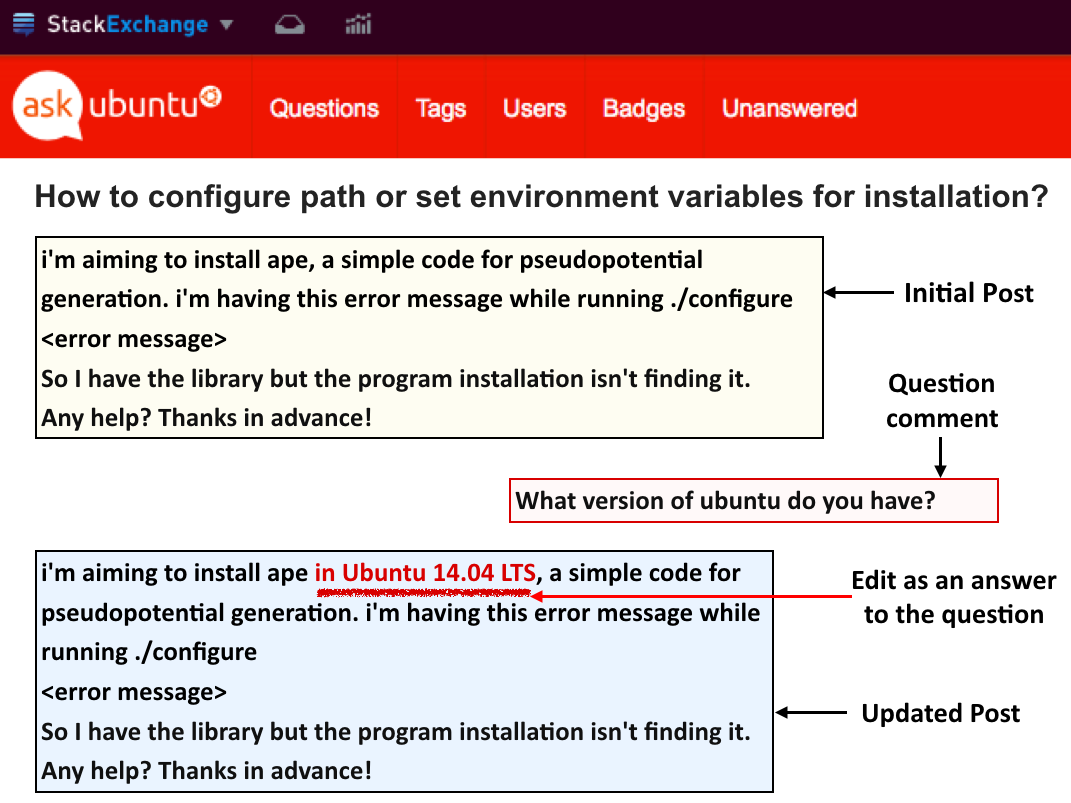
\includegraphics[width=0.47\textwidth]{askubuntu_post}}
\caption{A post on an online Q \& A forum ``askubuntu.com'' is updated to fill the missing information pointed out by the question comment}
\label{askubuntu_post}
\end{figure}
%
Our work has two main contributions: 
\begin{enumerate}[noitemsep,nolistsep]
%\item Identifying the problem of generating clarification questions as a problem worth of study, both in its own right and as part of the larger problem of building naturalistic conversational systems. 
\item A novel neural-network model for addressing this task that integrates the notion of expected value of perfect information (\S\ref{model}). % , a classic formalization from AI
\item A novel dataset, derived from StackExchange, that enables us to learn a model to ask clarifying questions by looking at the types of questions people ask (\S\ref{dataset_creation}).\footnote{We use data from StackExchange; per license cc-by-sa 3.0, the data is ``intended to be shared and remixed'' (with attribution). We will release all of the data we extract.}
\end{enumerate}

To develop our model we take inspiration from the decision theoretic framework of the Expected Value of Perfect Information (EVPI), a measure of the value of gathering additional information. In our setting, we use EVPI to calculate which question is most likely to elicit an answer that would make the post more informative.
Formally, for an input post $p$, we want to choose a question $q$ that maximizes $\mathbb{E}_{a \sim p,q}[\U(p+a)]$, where $a$ is a hypothetical answer and $U$ is a utility function measuring the \emph{completeness} of post $p$ if $a$ were to be added to it.
To achieve this, we construct two models:
(1) an answer model, which estimates $\mathbb{P}[a~|~p,q]$, the likelihood of receiving answer $a$ if one were to ask question $q$ on post $p$;
(2) a completeness model, $\U(p)$, which measures how complete a post is.
Given these two models, at prediction time we search over a shortlist of possible questions for that which maximizes the EVPI.

We are able to train these models jointly based on $(p,q,a)$ triples that we extract automatically from StackExchange.
Figure~\ref{askubuntu_post} depicts how we do this using StackExchange's edit history.  In the figure, the initial post fails to state what version of Ubuntu is being run. In response to Parker's question in the comments section, Terry, the author of the post, edits the post to answer Parker's clarification question. We extract the initial post as $p$, question posted in the comments section as $q$, and edit to the original post as answer $a$ to form our $(p,q,a)$ triples. 

Our results show significant improvements from using the EVPI formalism over both standard feedforward network architectures and bag-of-ngrams baselines, even when our system builds on strong information retrieval scaffolding. In comparison, without this scaffolding, the bag-of-ngrams model outperforms the feedforward network. We additionally analyze the difficulty of this task for non-expert humans, and give examples of system output. 

\begin{figure*}[t]
\centering
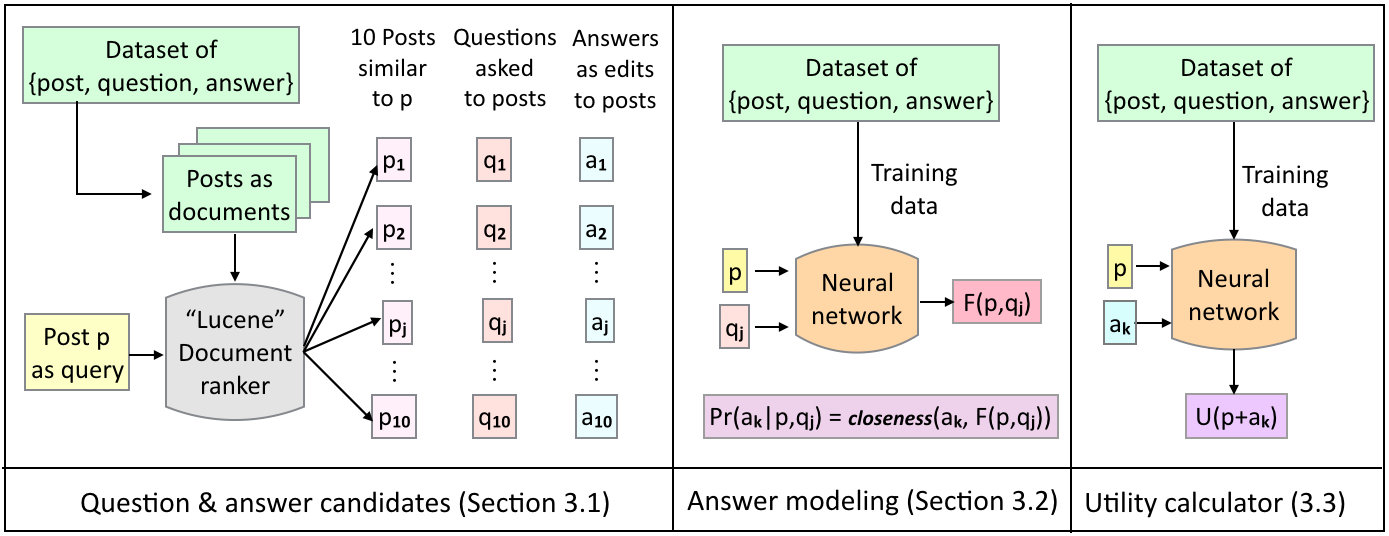
\includegraphics[width=0.85\textwidth]{model}
\caption{\small The behavior of our model during test time. Given a post $p$, Lucene retrieves 9 posts similar to post $p$ and consider the questions asked to those 9 posts, plus the original, as question candidates. The edits made to the posts in response to the questions as our answer candidates. For each question candidate $q_i$, we generate an answer representation $F(p,q_j)$ and calculate how close is the answer candidate $a_k$ to our answer representation $F(p,q_j)$. Our utility calculator calculates the utility of the post if it were updated with the answer $a_k$. Finally we return the question $q$ that maximizes the expected utility of the post $p$ (Equation~\ref{evpi_equation}).}
\label{model}
\end{figure*}

\section{Related Work} \label{related_work}

The problem of question generation has received sparse attention from the natural language processing community. Most prior work focuses on generating reading comprehension questions:  given text, write questions that one might find on a standardized test \cite{vanderwende2008importance,heilman2011automatic,rus2011question,olney2012question}.  Comprehension questions, by definition, are answerable from the provided text. Clarification questions are not.  

Outside reading comprehension questions, \newcite{labutov2015deep} generate high-level question templates by crowdsourcing and given a text segment, rank question templates that are relevant. However the crowdsourcing method of collecting data leads to significantly less data than we collect using our method. \newcite{liu2010automatic} use template question generation to help authors write better related work sections. \newcite{mostafazadeh2016generating} introduce a Visual Question Generation task where they consider question generation from images, a multi-modal variant of question generation. 
\newcite{penas2010filling} identify the notion of missing information similar to us but they attempt to fill the knowledge gaps in a text with the help of external knowledge bases, whereas we instead ask clarification questions. \newcite{artzi2011bootstrapping} use human-generated clarification questions to drive a semantic parser where the clarification questions are aimed towards simplifying a user query; whereas we generate clarification questions aimed at  identifying missing information in a text. 

\section{Model description}\label{model}

In order to choose what question to ask, we build a neural network model inspired by the theory of expected value of perfect information (EVPI). EVPI is a measurement of: if I were to acquire information X, how useful would that be to me? However, because we haven't acquired X yet, we have to take this quantity in expectation over all possible X, weighted by each X's likelihood. In the question generation setting, for any given question $q$ that we can ask, there is set $A$ of possible answers that could be given. For each possible answer $a \in A$, there is some probability of getting that answer, and some utility if that were the answer we got. The value of this question $q$ is the expected utility, over all possible answers. The theory of EVPI then states that we want to choose the question $q$ that maximizes:
\begin{equation}\label{evpi_equation}
\argmax_{q \in Q} \sum_{a \in A} \mathbb{P}[a | p,q] \U(p+a)
\end{equation} 

In Eq~\ref{evpi_equation}, $p$ is the post, $q$ is a potential question from a set of candidate questions $Q$ and $a$ is a potential answer from a set of candidate answers $A$. $\mathbb{P}[a | p,q]$ measures the probability of getting an answer $a$ given an initial post $p$ and a clarifying question $q$. $\U(p+a)$ is a utility function that measures how useful it would be if $p$ were augmented with answer $a$. In our case, the utility function we use is the completeness of the post: a post has high utility the more complete it is. This captures the right intuition in the example questions (from Section~\ref{introduction}) that Parker could have asked such that: \textsf{\small (a)} will have good utility for many likely answers;
\textsf{\small (b)} will have low utility regardless of the answer; and
\textsf{\small (c)} will have high utility only for a low probability answer.

The modeling question then is how to model: 
\begin{enumerate}[noitemsep,nolistsep]
\item the probability distribution $\mathbb{P}[a | p,q]$ and
\item the utility/completeness function $\U(p+a)$.
\end{enumerate}
In our work, both will be represented using neural networks over the appropriate inputs. Posts, questions and answers will all be represented as embeddings. We train the parameters of the two models jointly to minimize a joint loss defined such that an answer that has a higher potential of increasing the utility of a post gets a higher probability.

Figure~\ref{model} describes the behavior of our model during test time. 
Given a post $p$, our first step is to generate a set of candidate questions and a set of candidate answers (Section~\ref{question_candidate_generator}).
Given a post $p$ and a question candidate $q_i$, our second step is to calculate how likely is this question to be answered using one of our answer candidates $a_k$ (Section~\ref{answer_modeling}).
Given a post $p$ and an answer candidate $a_k$, the third step is to calculate the utility of the updated post i.e. $\U(p + a_k)$ (Section~\ref{utility_calculator})
Finally, using these pieces, we build a joint neural network that we can optimize end-to-end over our data (Section~\ref{neural_network}).

\subsection{Question \& answer candidate generator}\label{question_candidate_generator}

Given a post $p$, our first step is to generate a set of candidate questions and a set of candidate answers. One way that humans learn to ask questions is by looking at how others ask questions in a similar situation. Using this intuition we generate question candidates for a given post by identifying posts similar to the given post and then looking at the questions asked to those posts. For identifying similar posts, we use Lucene\footnote{\url{https://lucene.apache.org/}}, a software extensively used in information retrieval for extracting documents relevant to a given query from a pool of documents. Lucene also ranks the extracted documents according to their relevance to the query. We use Lucene to find the top 10 most similar posts to a given post from our dataset (Section~\ref{dataset_creation}) \footnote{The top most similar candidate to a post is the original post itself}. We consider the questions asked to these 10 posts as our set of question candidates and the edits made to the posts in response to the questions as our set of answer candidates. Section~\ref{dataset_creation} describes the process of extracting the (\textit{post, question, answer}) triples from the StackExchange datadump. 

\begin{figure*}[ht]
\centering
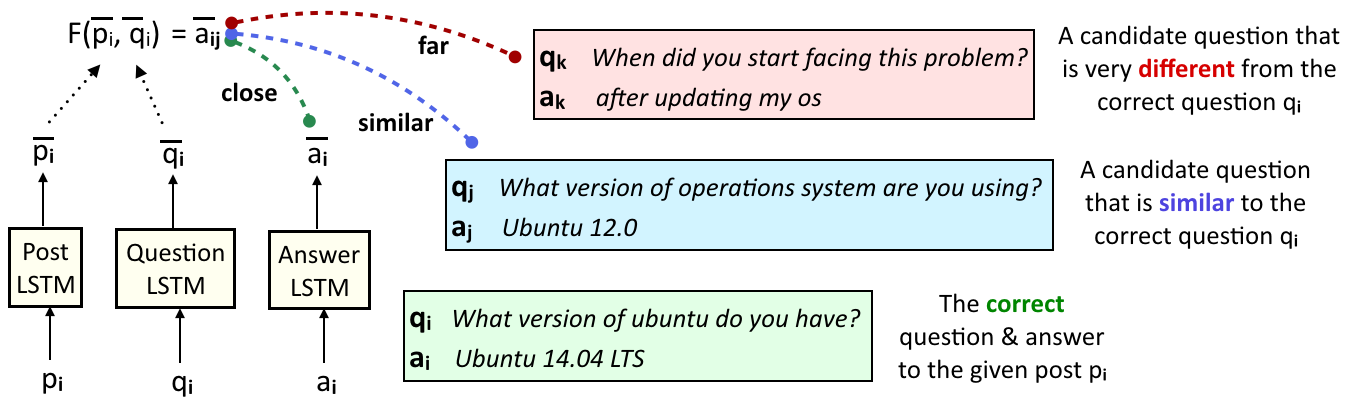
\includegraphics[width=0.9\textwidth]{answer_generator}
\caption{Training of our answer generator. Given a post $p_i$ and its question $q_i$, we generate an answer representation that is not only close to its correct answer $a_i$, but also close to one of its candidate answers $a_j$ if the candidate question $q_j$ is close to the true question $q_i$.}
\label{fig_answer_generator}
\end{figure*}

\subsection{Answer modeling}\label{answer_modeling}

Given a post $p$ and a question candidate $q_i$, our second step is to calculate how likely is this question to be answered using one of our answer candidates $a_k$. To calculate this probability, we first generate an answer representation using $p$ and $q_i$ and then measure how close is the answer candidate $a_k$ to our answer representation. To model our answer generator we use the following intuition: a question can be asked in several different ways. For e.g. in Figure~\ref{askubuntu_post}, the question ``\textsf{\small What version of Ubuntu do you have?}'' can be asked in other ways like ``\textsf{\small What version of operating system are you using?}'', ``\textsf{\small Version of OS?}", etc.  
Additionally, for a given post and a question, there can be several different answers to that question. For instance, ``\textsf{\small Ubuntu 14.04 LTS}", ``\textsf{\small Ubuntu 12.0}", ``\textsf{\small Ubuntu 9.0}", are all valid answers. We train our answer generator to generate an answer representation capturing these generalizations.

We use our dataset of \{\textit{post, question, answer}\} triples (Section~\ref{dataset_creation}). Given a $\{p_i, q_i, a_i\}$ triple, we use a long short-term memory architecture (LSTM) \cite{hochreiter1997long} to get to their respective neural hidden representations $\{\bar p_i, \bar q_i, \bar a_i\}$.  Given $(\bar p_i, \bar q_i)$, we define a feed-forward neural network $F$ that combines the post and question representations to get an answer representation $F(\bar p_i, \bar q_i)$. We train our answer generator to minimize the loss function below:
%
\begin{align}\label{eq_answer_generator}
  \textrm{loss}_{\textrm{ans}}(\bar p, \bar q, \bar a, Q) 
  &=  {|| F(\bar p, \bar q) - \bar a||}^2 & \\
  &\hspace{-25mm} +  \sum_{j \in Q} \Big ( {|| F(\bar p, \bar q) - \bar{a_j} ||}^2  (1 - \tanh{(|| \bar q - \bar{q_j} ||^2)}) \Big ) \Big \} &\nonumber
\end{align}
%
This loss function can be explained using the example in figure~\ref{fig_answer_generator}. Question $q_i$ is the question paired with the given post $p_i$. In equation~\ref{eq_answer_generator}, the first term forces the function $F(\bar p_i, \bar q_i)$ to generate an answer representation as close as possible to the correct answer $a_i$. Now, a question can be asked in several different ways. Let $Q_i$ be the set of candidate questions for post $p_i$, retrieved from the dataset using Lucene (Section~\ref{question_candidate_generator}). Suppose a question candidate $q_j$ is very similar to the correct question $q_i$ ( i.e. $|| \bar q_i - \bar{q_j} ||$ is near zero). Then the second term forces the answer representation $F(\bar p_i, \bar q_i)$ to be close to the answer $a_j$ corresponding to the question $q_j$ as well. Thus in the figure~\ref{fig_answer_generator}, the answer representation will be close to $a_j$ (since $q_j$ is similar to $q_i$), but far off from $a_k$ (since $q_k$ is dissimilar to $q_i$).

Given such an answer representation, we then define the probability distribution over candidate answers $a_k \in A$ as: 
\begin{align}
\mathbb{P}[a_k |p_i,q_j]  
&= \frac 1 Z \exp\left[- \lambda || a_k  -  F(p_i,q_j) ||^2\right]
\end{align}
where $\lambda$ is a tunable parameter that controls the variance of the distribution.

\subsection{Utility calculator}\label{utility_calculator}
Given a post $p$ and an answer candidate $a_k$, the third step is to calculate the utility of the updated post i.e. $\U(p + a_k)$. As expressed in equation~\ref{evpi_equation}, this utility function measures how useful it would be if a given post $p$ were augmented with an answer $a_k$. We train our utility calculator using our dataset of \{\textit{post, question, answer}\} triples (Section~\ref{dataset_creation}). We label all the $(p_i, a_i)$ pairs from our triples dataset with label $y=1$. To get negative samples, we make use of the answer candidates generated using Lucene as described in Section~\ref{question_candidate_generator}. For each $a_k \in A_i$, where $A_i$ is the set of answer candidates for post $p_i$, we label the pair $(p_i, a_k)$ with label $y=0$, except for when $a_k == a_i$. Thus, corresponding to each post $p_i$ in our triples dataset, we get one positive sample and nine negative samples. 

Given a post $p$ and an answer $a$, we use a post LSTM and an answer LSTM to get the neural representation $\bar{p}$ and $\bar{a}$. We define a feedforward neural network that combines the post neural representation $\bar{p}$ and the answer neural representation $\bar{a}$ to get the updated post representation $F(\bar{p}, \bar{a})$. The utility of the updated post is then defined as $\U(p+a) = \sigma ( F(\bar{p}, \bar{a}) )$. We want this utility to be close to 1 for all the positively labelled $(p,a)$ pairs and close to 0 for all the negatively labelled $(p, a)$ pairs. We therefore define our loss using the binary cross-entropy formulation below:
%
\begin{align}\label{eq_utility_calculator}
  \textrm{loss}_{\textrm{util}}(y, \bar p, \bar a) &= y \log(\sigma (F(\bar{p}, \bar{a})))
\end{align}

\subsection{Our joint neural network model}\label{neural_network}
Our fundamental representation is based on recurrent neural networks over word embeddings. We obtain the word embeddings using a GloVe \cite{pennington2014glove} model trained on the entire datadump of StackExchange. Given an initial post $p$, we generate a post neural representation $\bar{p}$ using a post LSTM i.e. long short-term memory architecture \cite{hochreiter1997long} as shown in the figure~\ref{lstm}. Similarly, given a question $q$ and an answer $a$, we generate a question neural representation $\bar{q}$ and a answer neural representation $\bar{a}$ using a question LSTM and an answer LSTM respectively. We define the function $F$ as a feedforward neural network on its input with two fully-connected hidden layers. So the function $F(\bar{p},\bar{q})$ in our answer model would be a feedforward neural network on the inputs $\bar{p}$ and $\bar{q}$ and the function $F(\bar{p}, \bar{a})$ in our utility calculator would be a feedforward neural network on the inputs $\bar{p}$ and $\bar{a}$. We train the parameters of the three LSTMs corresponding to $p$, $q$ and $a$, and the parameters of the two feedforward neural networks jointly to minimize the sum of the loss of our answer model (Eq~\ref{eq_answer_generator}) and our utility calculator (Eq~\ref{eq_utility_calculator}):
%
\begin{align}
                       \sum_i \textrm{loss}_{\textrm{ans}}(\bar p_i, \bar q_i, \bar a_i, Q_i)  
                        +  \textrm{loss}_{\textrm{util}}(y_i, \bar p_i, \bar a_i)
\end{align}
%
Given such an estimate $\mathbb{P}[a|p,q]$ of an answer and a utility $\U(p+a)$ of the updated post, predictions (i.e., selecting a question from a set of candidate questions) can be done by choosing that ``$q$'' that maximizes Eq~\ref{evpi_equation}. The remaining question, then, is how to get data that enables us to train our answer model and our utility calculator. Given data, the training becomes a multitask learning problem, where we learn simultaneously to predict utility and to estimate the probability of answers.

\begin{figure}
\centering
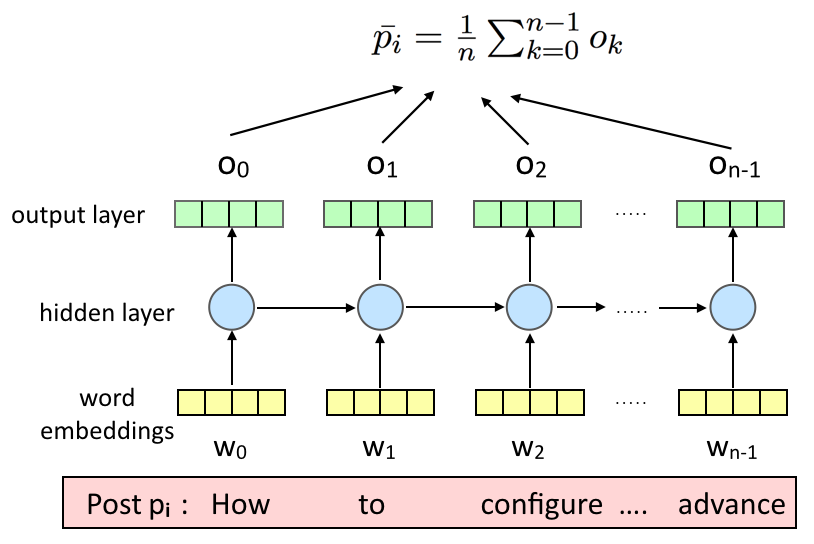
\includegraphics[scale=0.27]{lstm}
\caption{{\small Our LSTM architecture on a post $p_i$. The input layer consists of pre-trained word embeddings of the words in the post which is fed into a single hidden layer. The output $o_k$ of each of the hidden states is averaged together to get our neural representation $\bar p_i$}}
\label{lstm}
\end{figure}

\section{Dataset creation}\label{dataset_creation}
StackExchange is a network of online question answering websites about varied topics like academia, ubuntu operating system, latex, etc. The sites are modeled after StackOverflow, a popular platform used for asking and answering questions on a wide range of topics in computer programming. The data dump of StackExchange contains timestamped information about the posts, comments on the post and the history of the revisions made to the post. We use this data dump to create our dataset of \{\textit{post, question, answer}\} triples: where the \textit{post} is the initial unedited post, the \textit{question} is the comment containing a question and the \textit{answer} is the edit made to the post that matches the question comment. \\
\textbf{Extract posts:} We use the post histories to identify posts that have been updated by its author. We use the timestamp information to retrieve the initial unedited version of the post.\\
\textbf{Extract questions:} For each such initial version of the post, we use the timestamp information of its comments to identify the first comment made to the post. We look for a question mark `?' token to further identify if its a question comment. Finally, we truncate the comment till the question mark token to retrieve the question part of the comment.\\
\textbf{Extract answers:} In our final step, we identify the edit made to the post in response to the question comment. Authors make edits to their posts for several reasons; including stylistic updates and grammatical corrections. Therefore, we use only those edits that are longer than four words and finally use the timestamp information of the edit to match the edits to their respective question comments.

We extract a total of 38,041 (\textit{post, question, answer}) triples from StackExchange which are distributed across three domains: askubuntu (13,749), unix (6656), and superuser (17,636). We train our models using 80\% of the data, tune our hyper parameters using 10\% of the data and evaluate our models using the remaining 10\% of the data. Table~\ref{data_statistics} shows the sizes of the train, dev and test splits for the three domains. 

\begin{table}
\centering
\begin{tabular}{lccc}
\toprule
& Train & Dev & Test  \\
\midrule
askubuntu & 10,992 & 1374 & 1375\\
unix & ~~~5324 & ~~666 & ~~666 \\
superuser & 14,828 & 1404 & 1404 \\
\bottomrule
\end{tabular}
\label{data_statistics}
\caption{Table above shows the sizes of the train, dev and test split of our dataset for three domains.}
\end{table}

A natural question to our process of data creation would be how often is the extracted question a clarification question. We sample a set of 1400 questions from our dataset and design a crowdsourced task where given a question we ask a human to choose whether: a) It is a clarification question, b) It provides an answer or a suggestion; or c) Neither.  63\% of the questions are marked as clarification question, 33\% of them are marked as questions that provides an answer or a suggestion and 4\% of them are marked as neither. The inter-annotator agreement (PAA) is above 90\%. These numbers suggest that although a greater percentage of the extracted questions are clarification questions, our data is imperfect: it includes some non-clarification questions.

\section{Experimental Results}\label{experiments_results}
Our primary research questions that we evaluate experimentally are:
%
\begin{enumerate}[noitemsep,nolistsep]
\item Does a neural architecture with learned representations improve upon a simple bag-of-ngrams baseline?

\item Does the expected value of perfect information (EVPI) formalism provide leverage over a similarly expressive feed-forward network? %In particular, is EVPI a useful inductive bias for a model?

\item In the EVPI formulation, is it useful to compute an expectation over answers, rather than just picking a single question/answer pair?

\item How well does our model perform in comparison to non-expert humans?

\item How much harder is the task when the (distrator) candidate questions come from Lucene rather than selected randomly?\footnote{A common strategy with the Ubuntu dialogue corpus \cite{lowe2015ubuntu} is to train a dialogue system by choosing a best response given a context of a conversation and a set of candidate responses. However, these methods generate their candidates from their dataset using random sampling. This plausibly makes the task significantly easier than using Lucene to select candidates, which are much more likely to be confusable and have high lexical overlap.}
\end{enumerate}

\begin{table*}[t]
\small
\centering
\begin{tabular}{l|cccc|cccc}
\toprule
 & \multicolumn{4}{c|}{Lucene negative candidates} & \multicolumn{4}{c}{Random negative candidates} \\
Models & Acc & MRR & R@3 & R@5 & Acc & MRR & R@3 & R@5\\
\midrule
Random  & 10.0 & 29.3 & 30.0 & 50.0 &10.0 & 29.3 & 30.0 & 50.0 \\
Bag-of-ngrams & 11.6 & 31.3 & 32.5 & 54.6 & 54.9 & 70.5 & 83.1 & 92.0 \\
Feed-forward & 17.4 & 37.8 & 43.2 & 63.9 &  49.0 & 66.8 & 81.3 & 92.8 \\
EVPI max  & 21.1 & 41.2 & 48.0 & 66.9  & 48.8 & 65.5 & 77.2 & 89.9 \\
EVPI sum & \bf 23.3 & \bf 43.4 & \bf 51.0 & \bf 70.3 & \bf 61.1 & \bf 75.5 & \bf 87.9  & \bf 95.8  \\
\bottomrule
\end{tabular}
\label{results_topN}
\caption{Results of our two setups `Lucene negative candidates' and `Random negative candidates' on askubuntu test split when the model is trained on a combination of askubuntu, unix and superuser train splits}
\end{table*}


\subsection{Task setups}\label{task_setup}

\textbf{Lucene negative candidates:} In this setup, given a post $p$, we label the question $q$ paired with $p$ in our dataset of $(p, q, a)$ triples as positive. To get our negative candidates, we retrieve nine additional question candidates using Lucene (as described in Section~\ref{question_candidate_generator}).\\
\textbf{Random negative candidates:} In this setup, given a post $p$, we label the question $q$ paired with $p$ in our dataset of $(p, q, a)$ triples as positive as in the previous setting. To get our negative candidates, we randomly sample nine other questions from our dataset of $(p, q, a)$ triples.\footnote{In all cases we train 100-d word embeddings using GloVe \cite{pennington2014glove} on the 3 billion token datadump of StackExchange. We use a threshold frequency of 100 to create our vocabulary of ~250,000 tokens. For our feed-forward neural network, we use two fully-connected dense hidden layers each of size 100. We use ReLU \cite{nair2010rectified} non-linearity as our activation function between the hidden layers.}


\subsection{Baseline methods}\label{baselines}

We compare our model with the following baselines:\\
\textbf{Random baseline:} Given a post, we randomly permute its set of 10 candidate questions uniformly.\\
\textbf{Bag-of-ngrams baseline:} Given a post and a set of 10 question question and answer candidates, we construct a bag-of-ngrams representation for the post, the question and the answer. Our bag-of-ngrams baseline is then trained to minimize hinge loss on misclassification loss using cross-product features between each of (\textit{post, question}), (\textit{question, answer}) and (\textit{post, answer}). We tune the ngram length and the learning rate and choose the setting that performs best on development data.\\
\textbf{Neural network baseline using post, question and answer:} We concatenate the post LSTM representation, the question LSTM representation and the answer LSTM representation and feed it through a feed forward neural network of two fully-connected hidden layers to get our neural baseline. 

\subsection{Dataset}\label{dataset}
We evaluate our model and our baselines on the following three domains of StackExchange: askubuntu, unix and superuser.
 \begin{description}
 \item[askubuntu:]  A question and answer site for users of the Ubuntu Operating system where people post queries about issues they face while using Ubuntu. An example question on this site: ``\textsf{\small Why isn't Chromium up-to-date in all the Ubuntu LTS repos, like Firefox is?}''
 \item[unix:]  A question and answer site for users of Linux, FreeBSD and other unix-like operating systems. This site would contain questions like the ones in askubuntu and more. An example question on this site: ``\textsf{\small How to repeatedly alternate between two (or more) commands?}''
 \item[superuser:] A question and answer site for users of all kinds of operating systems and computer applications. An example question on this site: ``\textsf{\small What is the LAST version of Windows Operating system that can run DOS applications natively?}''
 \end{description}

Table~\ref{data_statistics} shows the data statistics for the four sites above.  Although StackExchange consists of many sites, we choose the ones above because: a) The data dump available for them were moderately big in size to train a model on; b) These domains contain clarifications questions that are generic enough to be useful for many different posts; and finally c) The three domains were close enough so that we could combine them to create our full dataset of ~37K triples.

\subsection{Results}

We first describe results on the union of all data, summarized in Table~\ref{results_topN}.
We report four metrics: accuracy (percent of time the top ranked question was correct),
mean reciprocal rank (the reciprocal of the ranked position in the top ten list that the correct question is), 
recall at 3 (percent of the the correct answer is in the top three) and
at 5.

The left half of this table shows results when the candidate sets is from Lucene---the ``hard'' setting.
Here, we see that for all the evaluation metrics:
EVPI using the sum (expectation over $a$) outperforms
EVPI using the max $a$;
which outperforms the neural feedforward model that does not incorporate the EVPI formalism;
which outperforms the bag-of-ngrams baseline;
which outperforms the random baseline.
The gains in all cases are relatively large: at least a few percentage points.
A final performance of 51\% recall at 3 is encouraging, though clearly there is a long way to go for a perfect system.

The right half of this table shows the same results when the candidate set is chosen randomly---the ``easy'' setting.
A major difference in the results here is that the bag-of-ngrams system now \emph{outperforms} both the feedforward neural model and the EVPI using max instead of expectation.
This likely happens because just picking up on word overlap---when Lucene has not already done this for us---works remarkably well.
Nonetheless, in all of the metrics, the true EVPI model outperforms all the baselines, achieving at least a 3\% gain over the bag-of-ngrams baseline.

In Table~\ref{results_topM} (supplementary materials), we show results when we work not with the union of all the data, but with each data set individually.
%The top half is against Lucene candidate, the bottom half is against random candidates.
The main observation is that the trends are essentially the same as before: for Lucene negative candidates, bag-of-ngrams underperforms feedfoward, which underperforms EVPI.
This happens because more data helps, and these three domains are sufficiently similar that the additional data---even if it is slightly domain mismatched---is better than nothing.
%The second observation is that the results for EVPI are lower across the board, with the exception of superuser on random negative examples.% (which is sometimes better, sometimes worse).

\subsection{How well can humans do this task?}

In this section we address two natural questions:
(1) how does the performance of our system compare to a human solving the same task?
(2) just because the system selects a question that is not the exact gold standard question, is it certainly wrong?
To answer these questions, we had 14 computer science graduate students perform an annotation task on $50$ examples.
Most of these graduate students are \emph{not} experts in unix or ubuntu, but all are knowledgable.
We provided them with a post and a randomized list of ten possible questions.
They were instructed to select what they thought was the \emph{single} best question to ask, and additionally mark as ``valid'' any additional questions that they thought would also be okay to ask.
We also asked annotators to rate their confidence in $\{0,1,2,3\}$.
Most found this task quite challenging because many of the questions are about subtle nuances of operating system behavior.

These annotator's accuracy on the ``hard'' task of Lucene-selected questions, was only 36\%, significantly better than our best system (23\%), but still far from perfect.
If we limited to those examples on which they were more confident (confidence of 2 or 3), their accuracy raised to 42\%, but never surpassed that.
A major problem for the human annotators is the amount of background knowledge required to solve this problem.
On an easier domain, or with annotators who are truly experts, we might expect these numbers to be higher.

The average number of ``valid'' answers for a single post according to the (admittedly non-expert) annotators was 4.26 (out of ten); the distribution was fairly symmetric and quickly decaying around that number (the median is four).
In the data, 56\% of the examples had at most four options marked as valid; 
28\% had at most 3; 14\% had at most 2; and 6\% had only one valid option (which by definition is also the ``best'' option).
These numbers suggest that an evaluation strategy that takes validity---and not just raw accuracy---is a useful avenue for future research.

\section{Conclusion}

We have described a new dataset for question generation, and attacked this problem from the perspective of question selection.
Our model integrates state-of-the-art neural network structure with the classic notion of expected value of perfect information, which effectively models a pragmatic choice on the part of the questioner: how do I \emph{imagine} the other party would answer if I were to ask this question. Such pragmatic priciples have recently been shown to be useful in other tasks as well \cite{golland2010game,smith2013learning,orita2015discourse,andreas2016reasoning}.

There are three main avenues for improvement of this work.
The first is in evaluation: given that this task is so difficult for humans, but also given that there is no single right question to ask, how can we better measure performance at this task?
This is exactly the same question faced in much research in dialog and generation more broadly \cite{paek2001empirical,lowe2015ubuntu,liu2016not,kannan2017adversarial}.
Second, to make question generation more general, systems need to be able to generalize, for instance by constructing templates of the from ``What version of \_\_\_ are you running?'' into which the system would need to fill a variable. Finally, asking question is a natural component of dialog, and building a collaborative dialog system that can naturally converse with a user is a broad long term goal.

\newpage

\chapter{Dialogue focus tracking for zero pronoun resolution}\label{dialogue_focus_tracking}

\section{Introduction}

``Pro-drop'' languages like Chinese, Japanese and Turkish allow for dropping of pronouns when the referents of those pronouns can be inferred. English is typically 
%\footnote{English requires subject pronouns to be dropped in imperative constructions; and in informal English, subject pronouns are sometimes optional.} 
\emph{not} pro-drop, but is unusual in that regard: two thirds of languages documented in WALS \cite{wals} can be categorized as pro-drop. In such languages, sentences are frequently characterized by ``zero pronouns'': gaps in the sentence which in English would hold an overt pronoun. In some languages, verbal morphology or clitics elsewhere in the sentence are sufficient to resolve the ambiguity of dropped pronouns; in other languages, there is \emph{no} overt marking at all in the sentence and the referent of the dropped pronoun must be resolved using pragmatic information.

\begin{figure}[t!]\label{sms-ex}
\centering
\includegraphics[width = .4\textwidth]{mainfig}
\caption{A conversation between a student and a teacher. The text has been translated from Mandarin, but zero pronouns are retained and indexed with their referent: (T)eacher or (S)tudent.}% Each utterance has a Focus, which is either the (T)eacher, the (S)tudent or (O)ther. These foci can be derived from a true English translation and are either (v)isible (overt in English) or (h)idden (assumed by focus coherence).}
\end{figure}

Our work departs from mainstream work on zero pronoun resolution in that we focus primarily on the resolution of \emph{deictic} zero pronouns. Unlike an \emph{anaphoric} zero pronoun (Section~\ref{ling}), whose reference must occur somewhere previously in the text, a deictic zero pronoun refers to a salient entity in the environment (such as the speaker, hearer or pragmatically accessible referent) without requiring introduction by an overt mention in the text. Although anaphoric zero pronoun resolution has been the focus of most past work \cite{yeh2007zero,chenchinese}, 50\% or fewer of zero pronouns in natural Chinese text are anaphoric \cite{zhao2007identification,kong2010tree}. Figure~\ref{sms-ex} shows an example conversation in which zero pronouns are frequently used to refer to speaker or listener, and would be translated to English as ``I'' or ``you.''

We propose a model for resolving deictic zero pronouns that draws inspiration from ideas in Centering Theory \cite{grosz1995centering}: discourses tend to settle on a particular \emph{focus} for a time, before switching. Furthermore, we presume that \emph{when} a switch happens, there is likely to be an overt cue of this. For example, in Figure~\ref{sms-ex}, the initial focus on \speaker{T} is signaled with the overt second person pronoun in the first utterance; the switch of focus to \speaker{S} in the third utterance is also signaled by an overt ``you.'' However, at that point, the focus remains on \speaker{S} for several utterances until ``The last round\dots'' at which point it switches away from the speakers. It is brought back to \speaker{S} in the last utterance, which can be inferred from the fact that \speaker{S} is the most recent focus that fits the required semantic constraints.

To account for these phenomena, \textbf{we develop a novel sequential model for zero pronoun resolution that explicitly tracks the conversation focus in a dialogue} (Section~\ref{focus_tracking_model}). We test, using data from Chinese SMS (``texting'') dialogues, the hypothesis that our model can predict the identity of pronouns (at a granularity of the person attribute: first, second, or third person---with particular focus on first and second person) based on a variety of features of the utterance context, without reference to a particular antecedent (Section~\ref{efficacy}). In this way, we address a much higher percentage of the zero pronouns found in Chinese texts, and particularly in dialogue.

Our second contribution is to show that \textbf{one can train a zero pronoun resolution system using supervision coming from English translations of the Chinese text} (Section~\ref{taa}). This obviates the need for expensive linguistic annotation of Chinese and allows us to use plentiful parallel data to train our model. Our results confirm that even though this ``translation as annotation'' process is noisy%\footnote{The noise is due to technical issues plus the fact that in informal settings, English \emph{does} allow some subject pronouns to be dropped.}
, it is still possible to learn on large amounts of ``bronze standard'' data.% than small amounts of ``gold standard'' data (Section~\ref{TODO}).

\section{Linguistic motivation} \label{ling}

Handling zero pronouns in Chinese (or other pro-drop language) involves two separate tasks: (1) Zero pronoun identification: locating and marking the gaps corresponding to zero pronouns; and (2) Zero pronoun resolution: determining the entity referred to by the zero pronoun. Our focus is the latter task.

Zero pronoun resolution, like general pronoun resolution, is almost universally approached as a problem of linking a pronoun to an overt noun phrase antecedent in the text. However, while some zero pronouns do have overt antecedents, many other zero pronouns do not. In fact, \cite{zhao2007identification} report that just 52\% of zero pronouns in their training set (and 46\% of zero pronouns in their test set) are ``anaphoric.'' Kong and Zhou \cite{kong2010tree} report just 41\%. Some zero pronouns fail to link to an antecedent because they refer to facts or events described by larger phrases or full sentences earlier in the text, preventing coreference with a single noun phrase. Other zero pronouns, particularly in dialogue settings, are \emph{deictic}, pointing to salient entities in the environment without requiring introduction by an overt mention in the text.% 

\subsection{Dialogue focus}

A central principle of document cohesion that underlies frameworks such as Centering Theory \cite{grosz1995centering} states that discourses tend to settle on a particular focus for a time, before eventually switching to a new one. The status of a particular focus within this flow of discourse is typically signaled by the form of the expression chosen to point to it. When a focus is introduced (or returned to), a full (overt) noun phrase is generally used to indicate it. While that entity remains in focus, subsequent mentions can be realized with less explicit forms. In English, these less explicit forms are overt pronouns. In Chinese (and pro-drop languages more generally), these focus continuations are generally realized as zero pronouns.

We see in this example an illustration of these discourse principles:
\begin{enumerate} \itemsep1pt \parskip0pt \parsep0pt
\item In pro-drop languages (Chinese), overt pronouns introduce switches in focus, while zero pronouns are used while an established focus continues.
\item In non-pro-drop languages (English), overt pronouns serve the focus-continuation function.
\item There are  ``non-anaphoric'' exceptions to these rules, licensed by environmental salience of the referent and inferable from the meaning of the utterance (final question of the example).
\end{enumerate}

Importantly, these continuations and switches of foci occur for the most part at the level of the syntactic clause. This is thus the level at which we model, assigning labels to individual clauses, which will in turn indicate the identity of any dropped subject pronoun in that clause.\footnote{Although Mandarin does license dropped object pronouns, we focus in this paper only on subject pronouns, as the syntactic subject is (a) more consistently dropped in Mandarin, and (b) more tightly tied to the notion of focus of conversation that motivates our model; see also a discussion of the centering hierarchy in Chinese \cite{chincent}.} In identifying focus, we remain at the granularity of the ``person'' attribute (first, second, or third person). This is the most relevant granularity for deictic pronoun resolution, as the intent is to capture the alternation between speakers within that dialogue (first and second person), along with switches of focus to any referents external to the dialogue (third person). %Number, gender, and animacy attributes are less likely to be captured by sequence labeling. 


\begin{table*}[t]
\begin{center}
\begin{footnotesize}
\begin{tabular}{|c|l|p{7cm}|c|}
\hline
                  & \bf Original Mandarin & \bf English Translation & \bf Label \\ 
\hline
1) \speaker{Student} & \includegraphics[height=0.8em]{conv-utt01.pdf} & How are you, Teacher Chen? & 2v \\
2) \speaker{Teacher} & \includegraphics[height=0.8em]{conv-utt02.pdf} & I am fine. You have not left yet?  & 1v, 2v\\
3) \speaker{Student} & \includegraphics[height=0.8em]{conv-utt03.pdf} & I have been back for a month.  & 1v, 1v \\
                  &                                                & I didn't dare to chat with you. & \\
4) \speaker{Student} & \includegraphics[height=0.8em]{conv-utt04.pdf} & Not yet.  & 1h \\
5) \speaker{Student} & \includegraphics[height=0.8em]{conv-utt05.pdf} & I have gone through 4 rounds of interviews for the American (company). & 1v \\
6) \speaker{Teacher} & \includegraphics[height=0.8em]{conv-utt06.pdf} & Why? & 2h \\
7) \speaker{Student} & \includegraphics[height=0.8em]{conv-utt07.pdf} & The last round of interview is with the general manager. & 3v \\
8) \speaker{Student} & \includegraphics[height=0.8em]{conv-utt08.pdf} & There are also two online tests. & 3h \\
9) \speaker{Teacher} & \includegraphics[height=0.8em]{conv-utt09.pdf} & Are you still in the interview phase? & 2v \\
\hline
\end{tabular}
\end{footnotesize}
\end{center}
\caption{Sample Chinese SMS conversation with English translation and derived labels.}
\label{conv}
\end{table*}

\subsection{Translation as annotation} \label{taa}

Currently, most state-of-the-art machine learning systems for Chinese zero pronoun resolution are supervised, requiring manually resolved pronouns for training.
We hypothesize comparable distribution between zero pronouns in a pro-drop language, and overt pronouns in a \emph{non}-pro-drop language. More specifically, because non-pro-drop languages lack zero pronouns, the discourse functions that are served by zero pronouns in pro-drop languages \emph{must} in non-pro-drop languages be served by overt pronouns.

To be more concrete, the original Mandarin SMS conversation from Figure~\ref{sms-ex} is reproduced in Table~\ref{conv}, together with a human translation into English.
Indeed, we see in the example in Figure~\ref{sms-ex} that the zero pronouns on the Chinese side correspond to overt pronouns on the English side. For this reason we make use of a parallel (Chinese/English) corpus for training of our sequence labeling model, deriving the identities of missing pronouns from the English translation of the Chinese text rather than from coreference relations with antecedents in the Chinese text. Our model thus does not rely on the availability of hand-annotated data for training. 

\section{Our focus tracking model}\label{focus_tracking_model}

Given a Chinese dialogue, our goal is to identify zero pronouns and resolve them either as deictic (first or second person) or anaphoric (third person). We use off-the-shelf tools for the identification of the zero pronouns (described in Section~\ref{setup}) and focus on the \emph{resolution} task.

In our implementation, we \emph{jointly} predict the \emph{focus} and identify the number of the pronoun that would be used. For instance, when \speaker{S} is speaking about herself, we consider this a ``\textbf{1}'' label; when \speaker{S} is speaking about her conversation partner, we consider this a ``\textbf{2}'' label. This numbering corresponds to which pronominal form would be required in English.\footnote{We ignore morphological issues in English dealing with possession and grammatical role, since these are exogenous to the resolution task.}

\subsection{Supervision via bronze standard data} \label{labels}

We obtain ``bronze'' standard (as opposed to ``gold'' standard) data by looking at human-produced English translations of Chinese utterances, such as those seen in Table~\ref{conv}. Our label set consists of two properties: the \emph{person} being referred to (first person, second person or third person), and whether the reference is overt or not (visible or hidden).
The ``visible'' three labels correspond to clauses in which an overt subject pronoun appears \emph{on the English side.} Chinese clauses bearing this label may have an overt or a zero pronoun subject---if the Chinese side contains a zero pronoun subject, then this label will be used to determine the correct person attribute (first, second, or third) of the unseen pronoun.

\begin{description} \itemsep1pt \parskip0pt \parsep0pt
\item[1v:] Overt English first person pronoun: ``I'' or ``we''
\item[2v:] Overt English second person pronoun: ``you''
\item[3v:] Overt English third person pronoun: ``he'', ``she'', ``it'', ``they'' 
\end{description}

However, there are plenty of utterances (e.g., 4 and 6) in which the English translation does not contain an overt subject. This can happen in English in imperative constructions, (some) questions, and general informal communication.\footnote{This can also happen due to imperfect zero pronoun identification (Section~\ref{setup}).}
%Due to a combination of imperfect automatic zero pronoun identification (described below), and subjectivity of Chinese-to-English translation, there are instances in the data in which an empty category has been identified in subject position on the Chinese side, but no overt subject pronoun appears on the English side.
In these cases, we introduce ``hidden'' person labels whose role is to carry forward the focus from the previous utterance. For instance, in utterance 4, even though there is no subject on the English side, we carry forward the fact that the most-recent referent was ``first person'' and denote this with ``1h.''

Because we are jointly modeling the focus shift and the pronoun realization aspects, when the speaker shifts, the ``hidden'' person must flip. For example, in utterance (5) the \speaker{Student} overtly refers to herself, yielding a label of ``1v.'' The next utterance is by the \speaker{Teacher} but lacks an English subject. The focus remains on the \speaker{Student} and therefore this utterance is labeled ``2h'' meaning that the focus is on the \emph{other} speaker, and it is non-overt in English.

%To deal with such discrepancies, we introduced the following labels (indicated by letter 'h', for 'hidden') to maintain the topic continuity encoded in the Subject continuation feature (explained in more detail in Section~\ref{features}) on the Chinese side, without attempting to link the identified empty category to a pronoun on the English side:
\begin{description} \itemsep1pt \parskip0pt \parsep0pt
\item[1h:] subject being continued is first person
\item[2h:] subject being continued is second person
\item[3h:] subject being continued is anything else 
\end{description}
Finally, we introduced a seventh label for instances in which no overt subject pronoun appears on the English side, and no focus has yet been established from prior clauses (this applies only at the beginning of a discourse). 
\begin{description} \itemsep1pt \parskip0pt \parsep0pt
\item[None:] no subject and no focus yet established
\end{description}
In Table 1, the rightmost column shows the label assignment for the sample SMS exchange. (The utterances on lines 2 and 3 contain two clauses each, and thus two labels each.)

\subsection{Features}\label{features}
We included in our model the following features. Note that these features are based solely on the \emph{Chinese side}. Linguistic motivations for each feature category are described.
%\begin{description} \itemsep1pt \parskip0pt \parsep0pt
\paragraph{Subject continuation:} a value indicating the \emph{person} (1, 2, 3) of the most recent overt NP that was a direct descendent of an IP node (the most recent overt NP in structural subject position---including, if overt, the subject of the current clause).  \emph{The most recent overt NP subject is a strong candidate for coreference with a zero pronoun. This feature comes closest to attempting antecedent selection.}
\vspace{-0.5em}

\paragraph{Verb:} the first verb in the VP that is sister to the subject NP (the VP of which that NP is the subject).   \emph{The nature of the verb can provide information relevant to inferring the identity of  deictic forms.}
\vspace{-0.5em}

\paragraph{Participant index:} a value indicating the index of the conversational participant.   \emph{To capture regularities, in any exist, in the pronoun use of a speaker.}
\vspace{-0.5em}

\paragraph{Participant switch:} a binary value indicating whether the current utterance represents a change of speaker relative to the previous clause.   \emph{Switches in speaker may, particularly in tandem with other features, be informative about topic.}
\vspace{-0.5em}

\paragraph{Object (downstream):} the direct object of the VP sister to the subject (if any).   \emph{This feature exploits the fact that pronouns occurring as direct objects within a clause cannot be the same as the (zero) pronoun in subject position of that clause.}
\vspace{-0.5em}

\paragraph{Has question particle:} a binary value indicating whether the clause contains a) a question particle or \emph{wh}-word, or b) a question mark.   \emph{This feature is likely to be a strong indicator of that the subject pronoun is \emph{not} first person (also used by \cite{chen2013chinese}).}
\vspace{-0.5em}

\paragraph{Bag of words:} all words occurring in the clause.   \emph{Apart from the verb, other words can also be highly informative about the nature of the subject.}
\vspace{-0.5em}

\paragraph{Bag of parts of speech:} all parts of speech occurring in the clause.   \emph{the structural make-up of clause may be informative about focus, for instance in the case of passive or possessive constructions.}
\vspace{-0.5em}

\paragraph{Hidden subject particles:} a feature indicating whether the clause consists of a list of phrases consistently tagged with empty categories on the Chinese side, but consistently translated without subjects pronouns on the English side (thus likely to correspond to labels 4-6).   \emph{This feature is intended to help the model in recognizing clauses consistently corresponding to ``hidden'' labels.}
%\end{description}

In addition for the features that consist of sequence (bag of words, bag of part of speech, object, etc.) we additionally compute bigrams and trigrams.

\subsection{Structured prediction}

We cast the above model as a sequence labeling problem over visible and hidden labels. We consider each conversation segment in the SMS as an input data sequence $\vec x = \langle x_1, x_2, \dots, x_n\rangle$ where each $x_i$ corresponds to a clause in Chinese. Each clause in Chinese is assigned a label from the label space $Y$ = \{1v, 2v, 3v, 1h, 2h, 3h, none\}. The task then is to assign labels $\vec y = \langle y_1, y_2, \dots, y_n\rangle$ to the input data sequence from the label space $Y$ based on the features described in Section ~\ref{features}. At training time we assign labels to the input sequence using the ``bronze standard'' method described in Section~\ref{labels}.

To train the sequence labeling model, we use an online variant of the DAgger imitation learning algorithm \cite{ross11dagger} as implemented in the Vowpal Wabbit machine learning library \cite{langford2007vowpal,daume2014efficient}. DAgger, like its predecessor \textsc{Searn} \cite{daume2009search}, solves structured prediction problems by transforming them into sequential decision making problems. In the case of sequence labeling, the natural order for sequence decision making is left-to-right. At test time, inference is performed greedily. At training time, the learning algorithm attempts to balance between training on ``oracle'' states (prefixes of decisions made optimally according to the true labels) and training on ``system'' states (prefixes of decisions made sub-optimally according to the learned model). The online variant of DAgger balances this trade-off by slowly transitioning from making past decisions optimally to making them using the currently learned predictor.

\section{Experiments} \label{focus_tracking_experiments}

Our goal in our experiments is to answer the following questions:

\begin{enumerate} \itemsep1pt \parskip0pt \parsep0pt
\item How well does the bronze-standard annotation capture the underlying truth? (Section~\ref{gold}).
\item Is our model able to leverage both dialogue structure and semantic content to accurately resolve pronouns? (Section~\ref{efficacy})
%\item Is ample bronze data more or less useful than meager gold data? (Section~\ref{loo})
\item How important are the different components in our model in making effective predictoins? (Section~\ref{ablation})
\end{enumerate}

In the following sections, we describe the experiments we perform aimed at answering these questions. First, we describe the data we use for experimentation.

\subsection{Experimental setup} \label{setup}

\begin{table}[t]
\begin{footnotesize}
\begin{center}
\begin{tabular}{|l|r|r|r|}
\hline
&
\multicolumn{1}{c|}{\bf Bronze} &
\multicolumn{1}{c|}{\bf SMS} &
\multicolumn{1}{c|}{\bf OntoNotes} \\
&
\multicolumn{1}{c|}{\bf Training} &
\multicolumn{1}{c|}{\bf Test} &
\multicolumn{1}{c|}{\bf Test} \\
\hline
\bf \# tokens & $1,007,722$ & $8104$ & $108,531$ \\ \hline
\bf \# sents  & $129,190$ & $1152$ & $9607$ \\ \hline
\bf \# dialog & $3309$ & $34$ & $257$ \\ \hline
\bf \# types  & $26,519$ & $1747$ & $4753$ \\ \hline
\end{tabular}
\end{center}
\end{footnotesize}
\caption{\label{dataset-numbers} Dataset statistics; numbers are for the Chinese side of the data. English has $25\%$ more tokens and roughly as many types.}
\end{table}

For training our focus-tracking model, we use Chinese-English parallel data from the SMS/chat domain available as part of training data used in the Machine Translation task under the BOLT project. The training data consisted of $117k$ sentences. We test our model on heldout SMS/Chat data consisting of $1152$ sentences, and on telephone conversation data from the OntoNotes corpus \cite{hovy2006ontonotes}, consisting of $5000$ sentences. Full data statistics are provided in Table~\ref{dataset-numbers}.

We perform zero pronoun identification using the method of \cite{cai2011language}, which automatically recovers empty categories corresponding to dropped pronouns, integrating these empty categories into syntactic parses. Syntactic parses were obtained with the Berkeley parser \cite{petrov2007improved}. These parses were then used to split the Chinese utterances into single-clause units, based on IP and CP clausal nodes. These clauses were aligned with clauses in the English translation, which were used to determine the identity of the clausal subject, for extracting the 1v,2v,\dots label for each utterance.\footnote{Sometimes English syntactic parses were not well-aligned with the Chinese IP/CP nodes; in practice, we split the English utterances based on end-of-clause punctuation and aligned Chinese and English clauses based on a simple order heuristic.}

For our machine learning systems, we use Vowpal Wabbit \cite{langford2007vowpal} with default hyperparameter settings. We train on $75\%$ of the trainind data and retain $25\%$ as development data on which to perform early stopping. We run 20 iterations by default and take the parameters with best development performance based on sequence labeling accuracy.

\subsection{Gold standard test set} \label{gold}

Although we can use ``bronze standard'' annotations for learning, evaluating against a bronze standard is not directly useful. Therefore, we annotated our test set ($1152$ utterances) by hand. In particular, for the SMS/chat test set, we recruited three linguistically-informed native Mandarin speakers to annotate Chinese clauses containing empty categories. The clauses were labeled with a person number (1,2,3) when the empty category corresponded to such a pronoun; or ``none'' in spurious cases.

In our annotated data\footnote{Annotations will be made freely available.}, $32\%$ of identified zero pronouns were first person, $17\%$ were second person, $25\%$ were third person and $26\%$ do not have a referent (were spurious). Of the correctly identified zero pronouns, a majority of pronouns (about 2/3) are deictic: referring either to the speaker or listener. The remainder are third person and mostly\footnote{In an in-person dialogue, a third person pronoun might be used in a deictic manner, as in ``\emph{She} is really smart'' while pointing at someone. This rarely occurs in SMS/chat because there is no shared environment beyond the two dialogue participants.} anaphoric.

\begin{table}
\begin{footnotesize}
\begin{center}
\begin{tabular}{|c|c|c|c|}
\hline \bf Pronoun & \bf Precision & \bf Recall & \bf F-measure \\ \hline 
\bf 1p & 0.75 & 0.43 & 0.55 \\ \hline
\bf 2p & 0.61 & 0.32 & 0.42 \\ \hline
\bf 3p & 0.52 & 0.45 & 0.49 \\ \hline
\bf Micro-avg & 0.62 & 0.41 & 0.50 \\ \hline
\end{tabular}
\end{center}
\end{footnotesize}
\caption{\label{bronze-vs-gold} Bronze vs Gold labels}
\end{table}

We then used these annotations to evaluate our bronze standard label assignment method against the gold standard judgments. Table~\ref{bronze-vs-gold} shows the precision, recall and F-measure of the bronze annotations when evaluated against the gold annotations. We can see a fairly significant discrepancy between our bronze labels and the gold labels. One major---and unfortunately inevitable---reason for this discrepancy is a high proportion of utterances in the English translation data which have been translated with the subject pronouns still absent. This is partially due to the casual nature of the text, and partially because the quality (fluency) of English translations in this data is at times dubious.

While there may be a systematicity to this kind of subject omission on the English side, this was not a factor taken into account by our human annotators. So while our own model may stand a chance at predicting ``hidden'' labels (no overt pronoun on English side) in such instances, the annotators will never assign a label of ``4'' to a location at which a pronoun could reasonably have been inserted.

\begin{table*}[t]
\begin{footnotesize}
\begin{center}
\begin{tabular}{|c|c|c|c|c|c|c|}
\hline
\multicolumn{7}{|c|}{\bf Subject Continuation Baseline} \\
\multicolumn{1}{|c|}{} & 
\multicolumn{3}{|c|}{\bf SMS Test set} & 
\multicolumn{3}{|c|}{\bf OntoNotes Test set} \\
\hline 
\bf Pronoun & \bf Precision & \bf Recall & \bf F-measure & \bf Precision & \bf Recall & \bf F-measure\\ \hline 
\bf 1p & 0.43 & 0.28 & 0.34 & 0.29 & 0.08 & 0.13 \\ \hline
\bf 2p & 0.27 & 0.19 & 0.22 & 0.28 & 0.11 & 0.16 \\ \hline
\bf 3p & 0.29 & 0.75 & 0.42 & 0.32 & 0.21 & 0.25 \\ \hline
\bf Micro-avg & 0.32 & 0.42 & 0.36 & 0.31 & 0.15 & 0.20 \\ \hline
\multicolumn{7}{c}{} \\
\hline
\multicolumn{7}{|c|}{\bf Our Full Model} \\
\multicolumn{1}{|c|}{} & 
\multicolumn{3}{|c|}{\bf SMS Test set} & 
\multicolumn{3}{|c|}{\bf OntoNotes Test set} \\
\hline
\bf Pronoun & \bf Precision & \bf Recall & \bf F-measure & \bf Precision & \bf Recall & \bf F-measure\\ \hline 
\bf 1p & 0.64 & 0.47 & 0.54 & 0.27 & 0.58 & 0.37 \\ \hline
\bf 2p & 0.55 & 0.21 & 0.31 & 0.25 & 0.23 & 0.24 \\ \hline
\bf 3p & 0.50 & 0.18 & 0.27 & 0.40 & 0.28 & 0.33 \\ \hline
\bf Micro-avg & 0.59 & 0.31 & 0.41 & 0.30 & 0.36 & 0.33 \\ \hline
\end{tabular}
\end{center}
\end{footnotesize}
\caption{\label{fullresults} Results across different pronoun categories for (top) subject continuation and (bottom) our full model.}
\end{table*}


\subsection{Overall system efficacy} \label{efficacy}

In this section we discuss the overall efficacy of our proposed method in comparison to a few alternatives. These alternatives are:

\paragraph{Random guessing baseline.}
A na\"ive system that makes predictions uniformly at random.

\paragraph{Subject continuation baseline.}
This is a rule-based approach that mimics the intuitions described in Section~\ref{ling}. In particular, for a Chinese utterance, we check whether the current utterance has an overt pronominal subject. If so, we assign a label of 1v, 2v or 3v depending on the person of this subject. If the current utterance has a non-pronominal subject, we assign 3h. Otherwise we ``carry forward'' the subject from the previous utterance, flipping the 1p/2p as necessary when the speaker changes; these are labeled as 1h, 2h or 3h.

\paragraph{Minimal model baseline.}
In the minimal model, we restrict our model to use just three features: participant index, participant switch and subject continuation feature. This is a machine learning variant of the rule-based subject continuation baseline.

\paragraph{Oracle upper bound.}
None of the proposed models can hope to achieve 100\% accuracy on this task because the Gold annotation data consists of $26\%$ ``no pronoun'' cases. Since all of our approaches \emph{must} predict a pronoun when a zero pronoun has been identified, their performance (namely, their precision) is upper-bounded away from $100\%$. 



\begin{table}[t]
\begin{footnotesize}
\begin{center}
\begin{tabular}{|l|c|c|c|c|c|c|}
\hline
                         & \multicolumn{3}{c|}{\bf SMS/chat}                          & \multicolumn{3}{c|}{\bf OntoNotes} \\
                         & \multicolumn{3}{c|}{\bf Micro-average}                 & \multicolumn{3}{c|}{\bf Micro-average} \\
\bf System               & \bf Pre & \bf Rec & \bf F & \bf Pre & \bf Rec & \bf F \\
\hline
    Random       & 0.24    & 0.25    & 0.24  & 0.18    & 0.26    & 0.22    \\
    Minimal         & 0.42    & 0.23    & 0.30  & 0.30    & 0.07    & 0.11    \\
    SubjCont & 0.32    & 0.42    & 0.36  & 0.31    & 0.15    & 0.20    \\
\bf Full Model           & 0.59    & 0.31    & 0.41  & 0.30    & 0.36    & 0.33    \\
    Upper Bound          & 0.74    & 1.00    & 0.85  & 0.55    & 1.00    & 0.71    \\
\hline
\end{tabular}
\end{center}
\end{footnotesize}
\caption{\label{summary-results} Summary of results for different comparator models against the gold standard labels from SMS data (left) and OntoNotes (right).}
\end{table}

The summary of results (micro-averaged across 1p, 2p and 3p) are shown in Table~\ref{summary-results}. These results show that on both the SMS data (on which the model was developed) and the OntoNotes data (on which the model was applied blindly), our full model is able to substantially outperform the baselines. In fact, on OntoNotes, despite a potential domain mismatch (from SMS/chat to telephone conversations), our full model was the only baseline to beat random guessing! Across both data sets, the minimal model tends to have high precision and low recall; the behavior of the other approaches varies across the tasks. On the SMS/chat data, our model achieves a $14\%$ relative improvement over the best baseline; on an OntoNotes data, a $50\%$ relative improvement.

More specific breakdowns of performance by different pronouns (1p, 2p and 3p) are shown for the subject continuation baseline and thefull model in Table~\ref{fullresults}. In these tables, we also report results when evaluated on the OntoNotes test set in these Tables. As we can see, the subject continuation baseline massively overpredicts third person pronouns in the SMS data, leading to an overall low score. In comparison, our model tends to have much higher precision (at the expense of recall) across the board on the SMS data, leading to a $14\%$ relative improvement over the subject continuation baseline.

Since no prior work (see Section~\ref{related-work}) has focused on deictic pronoun restoration, it is not possible to directly compare our results to previously published results. Although it is an apples-to-oranges comparison, a state-of-the-art \emph{anaphoric} zero pronoun resolution system \cite{chenchinese} achieves a precision of $13.3$, a recall of $32.2$ and an f-measure of $18.8$ on the \emph{full} OntoNotes data (our results are just for telephone conversations), but does so addressing the complementary problem of correctly choosing antecedents from previous overt noun phrases.

\subsection{Feature ablations} \label{ablation}

\begin{table}[t]
\begin{footnotesize}
\begin{center}
\begin{tabular}{|l|c|c|c|c|c|c|}
\hline
                         & \multicolumn{3}{c|}{\bf SMS/chat}                          & \multicolumn{3}{c|}{\bf OntoNotes} \\
                         & \multicolumn{3}{c|}{\bf Micro-average}                          & \multicolumn{3}{c|}{\bf Micro-average} \\
\bf System               & \bf Pre & \bf Rec & \bf F &\bf Pre & \bf Rec & \bf F \\
\hline
    Minimal (M)       & 0.42 	& 0.23 	& 0.30    & 0.30 	& 0.07 	& 0.11    \\
    M +  question 	& 0.44 & 0.23 & 0.30     & 0.31 & 0.07 & 0.12   \\
    M + object		& 0.43 & 0.23 & 0.30   & 0.30 & 0.07 & 0.12  \\
    M +  verb	           & 0.58 & 0.29 & 0.39    & 0.32 & 0.13 & 0.18    \\
    M + pos 		  & 0.52 & 0.30 & 0.38   & 0.23 & 0.27 & 0.25  \\
    M + bow		& 0.59 & 0.28 & 0.38 & 0.30 & 0.35 & 0.32  \\
    \bf Full Model           & 0.59    & 0.31    & 0.41    & 0.30    & 0.36    & 0.33    \\
\hline
\end{tabular}
\end{center}
\end{footnotesize}
\caption{\label{feature-ablation} Summary of results for feature ablation against the gold standard labels from SMS data (left) and OntoNotes (right).}
\end{table}

In order to investigate the individual contributions of each of our features, we performed feature ablation experiments, pairing our Minimal Model with a single feature at a time and retraining the model with this pairing. The results of these experiments can be seen in Table \ref{feature-ablation}.
We see in this table that for the SMS data, the Verb feature creates the greatest improvement over the Minimal Model, followed by Bag of Words and Bag of POS. This supports the hypothesis that the verb is informative with respect to the nature of its subject, as are the other words of the clause, and their parts of speech. For the OntoNotes corpus, however, the Bag of Words feature performs best by a large margin. Interesting, although the Bag of Words features are clearly the most useful, the linguistically motivated features (verb/question) performing well supports our linguistic intuitions.

\section{Discussion and prior work}\label{related-work}

Past approaches to zero pronoun resolution focus exclusively on anaphoric zero pronouns approached as a task of antecedent identification. Almost all work makes use of syntactic structure, with differences primarily in how that structure is used. \cite{yeh2007zero} take a rule-based, Centering Theory-inspired approach based on a system of constraints to guide selection of zero pronoun antecedents. In the same year, \cite{zhao2007identification} introduced a supervised learning approach for both zero pronoun identification and antecedent selection based on engineered features; these engineered features were replaced with a tree-kernel by \cite{kong2010tree}, who jointly perform zero pronoun identification, anaphoricity determination, and antecedent selection. Recently, \cite{chen2013chinese} built upon the model introduced by Zhao and Ng, introducing additional features and allowing coreference links between multiple zero pronouns. Chen and Ng (2013) also test their model on automatically identified zero pronouns and automatically generated parse trees, thus presenting the first end-to-end Chinese zero pronoun resolver. 

These approaches are mostly complementary to our task, since they focus on resolving anaphoric zero pronouns (the minority!) while we focus on resolving deictic zero pronouns. In particular, for a complete end-to-end system that resolves both deictic and anaphoric zero pronouns, one could first take our approach and whenever our model predicts ``third person,'' which is typically an anaphoric reference, one could apply one of these prior approaches.

The only work we are aware of that does not require linguistically annotated data for zero pronoun resolution is that of \cite{chenchinese}. They hypothesize that zero pronouns and overt pronouns have \emph{similar} distributions, and train an unsupervised model on \emph{overt} pronouns and then apply this model to \emph{zero} pronouns. This model performs on par with their previous (2013) supervised model. Despite this, their unsupervised model only agrees with their supervised model on 55\% of zero pronoun antecedents, suggesting that this hypothesis is weak.

In particular, the complementarity of zero versus overt pronoun usage has been studied within various domains of linguistics. The Position of Antecedent Hypothesis \cite{carminati2002processing} states that null and overt pronouns have different antecedent selection preferences: null pronouns prefer antecedents in subject positions, while overt pronouns prefer antecedents in non-subject positions. This hypothesis has been supported by studies in a variety of pro-drop languages (e.g., \cite{alonso2002null} \cite{kweon2011processing}). Switching of reference has been identified as one of the main constraints regulating use of zero versus overt pronouns in the variationist literature (see \cite{cameron1992pronominal} for sociolinguistic studies of the phenomenon in Spanish).% However these constraints on zero versus overt pronoun distribution have not been clearly captured and utilized in techniques for pronoun resolution and restoration. 

Our main result shows that although our bronze standard labels are noisy (Section~\ref{efficacy}), they are nonetheless for learning to resolve deictic pronouns. Moreover, one oft-heralded advantage of the translation-as-annotation scheme \cite{carpuat07psd} is that it naturally integrates into a machine translation framework, since one is learning to predict precisely what is necessary for successful translation; evaluating whether this hypothesis is true is currently an open question.


\newpage

\chapter{Selecting next response during two-way conversation}\label{dialogue_next_response}

\section{Introduction}

Data-driven methods for dialogue have experienced a recent surge in interest, due to a combination of the increasing availability of data and improved machine learning techniques.  To facilitate public research, \cite{lowe2015ubuntu} put together the Ubuntu Dialogue corpus by extracting two-way conversations from chat logs of discussions about issues with the Ubuntu Operating system. The task associated with the dataset is next utterance classification, given a portion of a conversation, and a set of possible next responses, identify the correct next response.

\begin{figure}[t]\label{sample_conversation}
\includegraphics[scale=0.45]{sample_conversation}
\caption{Sample conversation from Ubuntu Dialogue corpus. Terms \textit{`gnome', `menu', `debian'} are examples of topic words that occur in bursts. Terms \textit{`hackery', `shouldadd', `provding'} are examples of informal usage, elided whitespace and misspelling found frequently in this corpus.}
\vspace{-1.0em}
\end{figure}

Figure~\ref{sample_conversation} shows a sample conversation from the Ubuntu Dialogue corpus. We observe that word usage in such chat-based conversations differ from other domains. Firstly, topic specific words like \textit{`gnome', `menu', `debian'} occur in bursts within a conversation making them significant for the given conversation. However, these words are sometimes so rare in the entire corpus that they fall off the vocabulary threshold. To upweight such words, we introduce the idea of \textit{bursty vocabulary} (Section~\ref{bursty_vocabulary}) where the frequency of a word is defined by its count in the conversation where it occurs the most instead of its count in the corpus. We show that upweighting such bursty words helps a model distinguish the correct response from some random response. %like \textit{``on xchat an uparrow will bring up the last thing you typed.''} in the sample conversation in Figure~\ref{sample_conversation}

Secondly, due to the informal nature of these chats, they include several instances of misspellings, elided white spaces, abbreviations and informal usages. These and other character-level morphological variations in words cause issues when we use word-based representations. We introduce a character-level modeling approach called \textit{character trigram histogram} (Section~\ref{character_trigram_histogram}) where we append the one-hot vector representation of words with their character trigram histogram (Figure~\ref{fig:trigram_histogram}). We show that this approach facilitates statistical transfer between terms with small edit distance, thus reducing the representational differences between slightly varying words.

To evaluate our ideas, we conduct experiments on the Ubuntu Dialogue corpus where we start with the reference baseline model (Section~\ref{dataset_baseline}) described in \cite{lowe2015ubuntu} and apply modifications to it using ideas previously shown to be effective for dialogue modeling (attention aggregation and hierarchical modeling) to get a stronger baseline (Section~\ref{baseline_modifications}). We then show that our vocabulary redefining strategies, \textit{bursty vocabulary} and \textit{character trigram histogram}, give us significant improvements over the stronger baseline.  The simplicity of our approaches suggests general applicability for dialogue modeling. %Our contributions are inspired by best practices in language modeling, and their simplicity suggests general applicability for dialog modeling.

\section{Related Work} \label{related_work}

Following the introduction of the Ubuntu dialogue dataset, there has been several recent work that uses this dataset. 
\cite{lowe2015ubuntu} describe two neural network baseline models using Recurrent Neural Network (RNN) and Long Short Term Memory (LSTM). %\cite{hochreiter1997long}. 
\cite{kadlec2015improved} create an ensemble of LSTMs, Bi-LSTMs and Convolutional Neural Networks (CNN) to get improved baselines. 
\cite{xu2016incorporating} incorporate domain knowledge by enhancing their LSTM model with a recall gate.
\cite{baudivs2016sentence} introduce a unified approach for scoring sentence pairs %applicable to number of tasks including next utterance classification 
and show the current best result on the Ubuntu dialogue corpus task. 

The technique of attention aggregation (Section~\ref{attention_aggregation}) has been effectively used for several language based tasks like neural machine translation \cite{bahdanau2014neural}, \cite{luong2015effective}, question answering \cite{hermann2015teaching} and dialogue modeling \cite{yao2016attentional}. 
%More specifically in dialogue modeling, \cite{yao2016attentional} have shown that attending to the context while generating the words of the response gives an improvement over using just the last hidden state.
The technique of hierarchical modeling (Section~\ref{hierarchical_modeling}) was first introduced by \cite{serban2016hierarchical} as a latent hierarchical model where they add a context level RNN on top of token level RNN for processing sequences of sub-sequences.
\cite{serban2016multiresolution} take a similar approach but instead of defining a latent coarse representation, they assume it to be observed in the form of sequence of nouns and sequence of activities and entities
%\cite{serban2016multiresolution} take a similar approach but instead of defining a latent coarse representation, they assume it to be observed and experiment with two such representations (sequence of nouns and sequence of activities and entities).

%Ideas similar to bursty vocabulary have shown to be effective for neural machine translation. 
In the field of neural machine translation, there has been some work on vocabulary modifications for reducing the size of the large target vocabulary \cite{JeanCMB15, mi2016vocabulary} and for dealing with rare words \cite{luong2014addressing, sennrich2015neural}. 
%reducing the size of the large target vocabulary mainly for computational reasons \cite{JeanCMB15, mi2016vocabulary}. %\cite{DBLP:conf/acl/JeanCMB15} select a subset of words of the vocabulary via sampling, whereas \cite{mi2016vocabulary} introduce a sentence-level or a batch-level vocabulary. 
%\cite{sennrich2015neural} encode rare and unknown words as sequence of subword units and \cite{luong2014addressing} post process the out-of-vocabulary words in the translations using 
%\cite{DBLP:conf/acl/LuongSLVZ15}  -- for dealing with rare word note source word aligned to the OOV word and post process the output using a dictionary
%\cite{DBLP:conf/acl/JeanCMB15} -- select a subset of words of the vocabulary via sampling
%\cite{sennrich2015neural} encode rare and unknown words as sequence of subword units.
%\cite{mi2016vocabulary} introduce a sentence-level or batch-level vocabulary 
However, there has been no prior work that defines the vocabulary as we do for the purpose of dialogue modeling.
The character trigram histogram technique (Section~\ref{character_trigram_histogram}) was introduced as word hashing \cite{huang2013learning} to reduce the dimensionality of bag-of-words term vectors. We, on the other hand, find its use in normalizing over character level differences by enhancing the word-level representation with the character trigram histogram. 

\section{Dataset and Baseline Model}\label{dataset_baseline}

The Ubuntu dialogue corpus is a collection of one million two person conversations systematically extracted from chat log of forums where people discuss issues related to the ubuntu operating system. The task associated with the dataset is next utterance classification, which facilitates assessment while remaining plausibly related to more
complex design goals.  The problem, given a portion of a conversation (\textit{context} in Figure~\ref{sample_conversation}), and a set of possible next responses, is to identify the correct next response (\textit{response} in Figure~\ref{sample_conversation}).  The set of possible next responses includes the true continuation of the conversation as well as negative distractor utterances randomly sampled from the corpus.

We use the best reference model provided with the dataset as our starting point which is a siamese network of two LSTMs, one for context and one for response, with tied weights. The words of the context (and response) is fed into the LSTM one word at a time. The final hidden state of the two LSTMs represent the summary of the input context and the response respectively and the model is trained to minimize the cross entropy of all labelled context, response pairs.

\section{Baseline Modifications}\label{baseline_modifications}

\subsection{Attention Aggregation}\label{attention_aggregation}

The baseline model described before uses the last hidden state of the LSTM to represent the input. Our experiments indicate that a simple averaging of the hidden states gives an improvement over using just the last state. We achieve a further improvement with a simple attention mechanism. % by taking a weighted average over the hidden states where the weights are learned during training.  
%The idea of attending to some part of the input more than the other was first used for translation \cite{bahdanau2014neural}. %where the probability of predicting a certain word on the target side was conditioned on a distinct context on the source side. 
%In dialogue modeling, 
\cite{yao2016attentional} show that attending to the context while generating the words of the response gives an improvement over using just the last hidden state. On similar lines, we use the notion of soft-attention where we take a weighted average over the hidden states and learn those weights during training. 

\subsection{Hierarchical Modeling}\label{hierarchical_modeling}

Conversation between two people proceeds via utterances such that each utterance defines a message in itself and the utterances together define the conversation. To model this hierarchy, we define a token level LSTM that operates on the tokens and an utterance level LSTM that operates on the utterances. Hidden states from token-level LSTM are aggregated using attention to get utterance level representations which are then fed to an utterance level LSTM. Hidden states from utterance level LSTM are finally aggregated using attention to represent the input. %Hierarchical modeling techniques similar to ours have been shown to be effective for dialogue modeling \cite{serban2016hierarchical}, \cite{tranhierarchical}.

\section{Our Vocabulary Redefining Methods}\label{our_methods}

\subsection{Bursty Vocabulary}\label{bursty_vocabulary}

Models that use vector representations for words often define the vocabulary using a cut-off on the frequencies of words in the entire corpus, replacing all lower frequency words with a special out-of-vocabulary token. As is typical with power law statistics, there are a large number of infrequently occurring tokens in the Ubuntu Dialogue corpus e.g., due to misspellings and incorrect tokenization.  Cross validation indicates the optimal frequency cutoff for this dataset is actually quite high, e.g., including tokens with a total count below 20 leads to overfitting. 
However, these rare terms include tokens that are only used in a few conversations, but which occur at a high frequency within these conversations.  Intuitively this could correspond to rare entities that are the topic of a few conversations, and which would be  highly discriminative for next utterance classification. To upweight such words, we define the following notion of a bursty vocabulary: the frequency of a word is defined by its count in the conversation where it occurs the most and a vocabulary is thereafter defined using a cut-off on these word frequencies.  Experimentally this simple approach is surprisingly effective.

To understand the idea of bursty vocabulary better, we inspect words from our corpus that were included in the bursty vocabulary and excluded in the regular vocabulary and vice-versa. We call them bursty non-frequent words and frequent non-bursty words respectively. Some examples of bursty non-frequent words are \textit{`multicasting', `techsupport',} and  \textit{`mutex'}; suggesting bursty words are rare topic words. We find that 32\% of the words in our bursty vocabulary fall out of our regular vocabulary.
When we looked at the conversations where these words occurred the most we found that they corresponded to conversations where the speakers were talking about an issue with say multicasting, techsupport or mutex; these words were likely to occur in the true next utterance but not in the distractor utterances.
Some examples of frequent non-bursty words are \textit{`insulting', `accurate'} and \textit{`baggage'}; suggesting that frequent words may not correspond to topic words, and therefore may be less useful for identifying the true next response. We find that 57\% of our regular vocabulary are non-bursty words.

\begin{figure}
\includegraphics[scale=0.3]{trigram_histogram}
\caption{Character trigram histogram for an example word \textit{``bananas''}}
\label{fig:trigram_histogram}
\vspace{-1.0em}
\end{figure}

\begin{table*}
\begin{tabular}{  c | c | c | c | c | c | c | c | c }
Model & TF-IDF & RNN & LSTM & +Attn & +Hierar & +Bursty & +TrigHist & RNN-CNN \\ \hline
1 in 2 R@1 & 0.749 & 0.777 & 0.869 & 0.874 & 0.887 & 0.892 & \textbf{0.916} & 0.911\\ 
1 in 10 R@1 & 0.488 & 0.379 & 0.552 & 0.606 & 0.621 & 0.633 & \textbf{0.644} & 0.672\\
1 in 10 R@2 & 0.587 & 0.561 & 0.721 & 0.773 & 0.783 & 0.793 & \textbf{0.805} & 0.809\\ 
1 in 10 R@5 & 0.763 & 0.836 & 0.924 & 0.953 & 0.954 & 0.956 & \textbf{0.961} & 0.956 \\ \hline
\end{tabular}
\caption{Results on the test set of Ubuntu Dialogue dataset reported in Recall. The first three columns correspond to the baseline models described in \cite{lowe2015ubuntu}. Attention aggregation (Attn) and Hierarchical modeling (Hierar) are our modifications to the LSTM baseline. Bursty vocabulary selection (Bursty) and Character trigram histograms (TrigHist) are our vocabulary redefining models. The last column corresponds to the RNN-CNN model reported in \cite{baudivs2016sentence} which is the current state-of-the-art on this dataset.}
\label{results}
\end{table*}

\subsection{Character Trigram Histogram} \label{character_trigram_histogram}


Most modeling of text for various natural language processing tasks have been done at the word level. Recent work in neural machine translation has seen the benefit of modeling at a sub-word level. This can be especially useful for natural dialog due to phenomena such as misspellings, elided white spaces, and abbreviation. We found character trigram histograms to be simple and highly effective. Figure \ref{fig:trigram_histogram} shows a sample trigram histogram of the word \textit{bananas}. The left column lists all the trigrams in the word and their frequencies.  Associated with each trigram is an index: a trigram which occurs sufficiently frequently in the training corpus is assigned a unique index, and all other trigrams are assigned the special out-of-trigram index. The trigram histogram for each word is then defined as a frequency vector of size of the trigram vocabulary.  
We reduce the dimensionality of the trigram histogram vector using Principal component analysis (PCA) \cite{tipping1999probabilistic} and concatenate it with the word embedding to get our final word representation. The representations of two words that have small edit distance will have larger inner product, thus facilitating statistical transfer between them.
This yields two interesting properties.  First, the representations for two tail tokens that have small edit distance will have larger inner product than if the edit distance were large, facilitating statistical transfer between tail terms of low edit distance.  Second, the use of dropout on the input variables will facilitate statistical transfer between head terms and tail terms with small edit distance, as the one-hot portion of the representation will sometimes be dropped out.

\section{Experiments and Results}\label{ubuntu_experiments_results}

We evaluate our models on the Ubuntu Dialogue corpus\footnote{We use version 2 of the dataset where negative sampling is not uniform, thus increasing the difficulty of identifying the next utterance.} which consists of one million dialogues. Out of this 2\% is set aside as the test set, 2\% as the validation set and the rest is used for training. The task is set up as a ranking task where given $n$ responses, a system's ranking is considered as correct if the correct response is among the first $k$ candidates. We report recall values with $(n,k)$ as $(2,1), (10, 1), (10, 2)$ and $(10, 5)$. 

\subsection{Experimental Details}
We implement our models\footnote{Our code is available on \href{http://github.com/raosudha89/ubuntu_dialogue}{github} } using the Lasagne \cite{lasagne} library. For all our LSTM based models and its variations, we limit the number of context and response tokens to 100 and use a single hidden layer of size 300. We use Adam \cite{kingma2014adam} as our optimizer, with gradients clipped to 10. 

For representing a word, we use word embeddings of size 300 which are initialized using the pre-trained GloVe vectors (Common Crawl, 840B tokens \cite{pennington2014glove}) and fine-tuned during training. Words in the corpus not included in the pre-trained model are initialized randomly using uniform sampling from [-0.25, +0.25] to match the embedding standard deviation. 

For our character trigram histogram model, we further append the word embedding with a trigram histogram embedding of size 50 %(obtained by PCA on the trigram histogram frequency vector). 
We use a frequency threshold of 15 for our regular vocabulary and 3 for our bursty vocabulary.  

\subsection{Results}
Table~\ref{results} compares the performances of different models. We obtain results by incrementally adding each of our methods to the LSTM baseline model described in \cite{lowe2015ubuntu} such that the `+TrigHist' column corresponds to our final model which is a combination of all our methods.
%The recall values steadily increase from left to right
%TF-IDF, RNN and LSTM are the baseline models described in \cite{lowe2015ubuntu}. 
%Columns with prefix `+' in their heading should be read as the incremental results obtained by the addition of current model to all the previous models starting from the LSTM baseline such that the `+TrigHist' column corresponds to our final model. 
%The last column corresponds to state-of-the-art \cite{baudivs2016sentence} on this dataset which is a combination of recurrent and convolutional neural networks (RNN-CNN). 
The results show that our \textit{bursty vocabulary}  and \textit{character trigram histogram} strategies together achieve a 3\% improvement over the strong LSTM+attention+hierarchical baseline and are comparable to the state-of-the-art model. 

\section{Conclusion}

In this work, we introduce two strategies for redefining the vocabulary to make it more conducive to a dialogue environment. By upweighting words that occur in bursts within a conversation, our \textit{bursty vocabulary} strategy redirects the focus of a model from frequent words to topical words. By modeling character level information, our \textit{character trigram histogram} strategy helps bin slightly varying words together thus overlooking issues like misspellings, elided white spaces, abbreviations and informal word variations found frequently in dialogues. 

%In future, we plan to apply our methods to other tasks that use dialogue-like data (e.g. twitter, online community question answering, etc). 
Although our methods have been inspired by the atypical word usage in dialogues, we can apply them to other scenarios where such rare word modeling could be useful; for e.g. machine translation, community based question answering on \textit{StackExchange, Reddit}, or any task that make use informal data such as \textit{Twitter, Facebook or SMS}.

\newpage

\chapter{Proposed Work}\label{proposed_work}

\section{Template based question generation}

In our preliminary work, we focused on the question selection problem i.e. select the right clarification question from a set of prior questions. To make the system more general, it needs to be able to generalize to unseen context well. For e.g. consider a scenario in which the post is talking about the application `apt-get' that the model has never seen in its past before. However, from the context, it can make out that the discussion is similar to a different discussion where the topic was the application `yum' and a plausible clarification question is asking for the version of the application. However, since it has not seen a clarification question like ``What version of yum are you using?'', it fails to generate one. To circumvent this generalization issue, we propose a template based question generation method. For instance, consider a template like ``What version of \_\_\_  are you running?''. This template can generate thousands of specific variants found in the data like ``What version of Ubuntu are you running?'', ``What version of OS are you running?'', ``What version of apt-get are you running?'', etc. We enumerate four steps of our template based question generation method:

\begin{enumerate}
\item Identify groups of similar questions from a huge collection of questions.
\item Generate a template for each group of questions.
\item Given a post, select a question template from a set of candidate question templates.
\item Fill in the variables in the template using words relevant to the given post.
\end{enumerate}

\noindent
For grouping similar questions together, we plan to explore some of the clustering algorithms which cluster documents based on their lexical and semantic similarity. A preliminary experiment of trying to cluster questions has revealed that the questions are too different from each other to form useful clusters. We therefore propose a different strategy in which we will remove topic specific words from the questions and then cluster them, thus forcing a generalization before grouping them. To generate templates corresponding to each cluster, we plan to further identify topic specific words from the question using syntactic information (like parts-of-speech tags) and then remove them to form generic templates. In the third step, given a post and a set of candidate question templates, we will select a template using a model similar to our clarification question selection model described in our preliminary work in Chapter~\ref{stackexchange}. Finally, in the fourth step, we will fill in the blanks in the template with topic specific words from the post. We plan to first generate a candidate set of topic words from the post and then train a machine learning model which given the context of the post and the question template would select the correct topic word from the candidate set of topic words.
%plan to explore methods similar to slot filling approaches \cite{} to populate the blanks in the template with post specific words.
 
\newpage
\section{Sequence-to-sequence based question generation}

Sequence-to-sequence neural network models have proven to be effective for several language generation tasks like machine translation (Sutskever et.al. 2014), dialog generation (Serban, Iulian V., et al. 2016), etc. The main idea behind these models is that they work on an encoder-decoder framework. The encoder model takes in the words of the input one word at a time, passes it through a recurrent neural network (or its variants like LSTM, GRU, etc) and generates a final vector representation of the input. The decoder, then, takes in this input representation and a start symbol and generates the words of the output one word at a time till it generates the end of sequence symbol. The model is trained using a large number of input/output sequences to minimize the perplexity between the generated output sequence and the true output sequence.\\

\noindent
On similar lines, we propose a model for generating the clarification question one word at a time, given the words of a post. A recent neural generative question answering model \cite{yin2016neural} built an answer language model which decides, at each time step, whether to generate a common vocabulary word or an answer word retrieved from a knowledge base. Thus the model is built on an encoder-decoder framework equipped with the ability to enquire a knowledge base of facts contained in the form of entity-relationship triples. Inspired from this work, we propose to build a question generation model which will decide, at each time step, whether to generate a common vocabulary word or a topic specific word retrieved from the current post. Using this approach we thus incorporate the template based question generation method into a more general neural network framework.

\section{Clarification questions for dialog systems}

In our preliminary work we developed a model for generating a clarification question in a non-interactive setting i.e. after someone has described their problem in its entirety, we ask a question. However, most of such problem solving happens in the form of a dialog between a system and a human. In our next research direction, we propose to build a model that learns to generate  clarification questions at different stages of an ongoing conversation. Our model will learn the trade-off between asking a generic question at the initial stages and asking a specific question at the later stages of a conversation. We will define a cost function that measures the worth of asking a question at an early stage versus at a later stage. \\

\noindent
For the dataset, we plan to use the Ubuntu Dialogue corpus, a large corpus recently put together by \cite{lowe2015ubuntu} by extracting two-way conversations from chat logs where people were discussing about the issues they were having with the Ubuntu Operating system. In our preliminary work (Chapter~\ref{dialogue_next_response}), we defined a model that selects the next best response given the context of a conversation. We find that, given the problem solving domain of these chats, many of these responses are questions. Therefore, we plan to define our task as, given the context of a conversation, decide whether there is value in generating a clarification question as the next response and if there is some value, ask the question. We will use different lengths of context of a single conversation to compare the value of generating a clarification question early on in a conversation with little context and the value of waiting and generating a clarification question later on in the conversation with more context. 

\newpage
\section{Identifying missing information using knowledge bases}

In the approaches described so far, the models learn to ask a clarification question by looking at previously asked questions in a similar context. More specifically, we rely on our data to include the kinds of questions that we would like to ask. The main purpose of generating the clarification questions is to identify the missing information in a given text. To understand what is missing, one needs to first know what should have been there. As humans, we rely on our prior knowledge about the subject to decide what should have been there but is missing and then ask a clarification question pointing out the missing information. \\

\noindent
Therefore, in our last proposed work, we propose to develop a model which extracts information from knowledge sources like Wikipedia and makes use of it to generate clarification question. Sites like academia, music, mythology, etc on StackExchange contain discussions which require domain knowledge readily available on Wikipedia. We propose the following four-step approach to our knowledge base induced clarification question generator:
\begin{enumerate}
\item Given a post on StackExchange, we will first extract a Wikipedia page that is most relevant to the given post.
\item In the second step, we will use the structured information on the Wikipedia page to extract the attributes of the topic of discussion in the post. For instance, in the domain of music, the topic "song" would contains attributes like singer, genre, album, etc.
\item In the third step, we develop a method to identify which of the attributes extracted in the previous step are currently missing in the given post.
\item Finally, in the fourth step, we will generate a question that would ask about the missing attribute identified in the previous step.
\end{enumerate}


\newpage

\chapter{Conclusion and Timeline}\label{conclusion}

In this proposal, we identify that the problem of generating clarification questions is a problem worth of study, both in its own right and as part of the larger problem of building naturalistic conversational systems. To our knowledge, this is the first time a work has focused solely on generating clarification questions. We present our preliminary work on generating clarification questions on StackExchange posts and propose methods to generalize this approach further to new contexts. We present our work on dialogue focus tracking and its application on the task of zero-pronoun resolution. We present our preliminary work on identifying the next best response given the context of a conversation and propose methods to specifically generate clarification questions in the context of dialogues. Finally, we propose a novel method that makes use of external knowledge bases to identify missing information before it generates a question, thus bridging the gap between pure corpus driven approaches and pure knowledge base driven approaches for question generation. 

\section{Timeline}

The timeline for my proposed work is as follows:
\begin{itemize}
\item 2017-05: Proposal
\item 2017-09: Template based question generation
\item 2017-11: Sequence to sequence based question generation
\item 2018-01: Clarification questions for dialogues
\item 2018-04: Identifying missing information using knowledge bases
\item 2018-06: Thesis
\item 2018-07: Defense
\end{itemize}

\begin{small}
\bibliographystyle{acl_natbib}
\bibliography{proposal}
\end{small}

\end{document}


